\documentclass[conference]{IEEEtran}

\usepackage[utf8]{inputenc}
\usepackage[T5]{fontenc}
\usepackage{amsmath,amssymb}
\usepackage{booktabs}
\usepackage{multirow}
\usepackage{array}
\usepackage{tabularx}
\usepackage{xcolor}
\usepackage{graphicx}
\usepackage{tikz}
\usetikzlibrary{arrows.meta,positioning,fit,calc,shapes.geometric,backgrounds}
\usepackage{algorithm}
\usepackage{algpseudocode}
\usepackage{url}
\usepackage[hidelinks]{hyperref}

\newcommand{\sys}{AIC26-Retrieval}
\newcommand{\kis}{KIS}
\newcommand{\trake}{TRAKE}
\newcommand{\rrf}{RRF}
\newcommand{\sid}{\texttt{submit\_keyframe\_id}}
\newcommand{\vid}{\texttt{video\_id}}
\newcommand{\fid}{\texttt{frame\_idx}}
\newcommand{\kfn}{\texttt{keyframe\_n}}
\newcommand{\ptstime}{\texttt{pts\_time}}
\newcommand{\submitpair}{\texttt{video\_id + frame\_idx}}
\newcommand{\field}[1]{\nolinkurl{#1}}
\newcommand{\etal}{\emph{et al.}}

\definecolor{aicblue}{RGB}{41,98,255}
\definecolor{aiccyan}{RGB}{0,137,167}
\definecolor{aicgreen}{RGB}{46,125,50}
\definecolor{aicorange}{RGB}{239,108,0}
\definecolor{aicred}{RGB}{198,40,40}
\definecolor{aicgray}{RGB}{84,98,111}
\definecolor{aiclight}{RGB}{244,247,251}

\tikzset{
  block/.style={draw, rounded corners=2pt, thick, align=center, font=\scriptsize,
    minimum height=7mm, text width=25mm, fill=aiclight},
  wideblock/.style={draw, rounded corners=2pt, thick, align=center, font=\scriptsize,
    minimum height=8mm, text width=36mm, fill=aiclight},
  db/.style={draw, cylinder, shape border rotate=90, aspect=0.22, thick,
    align=center, font=\scriptsize, minimum height=9mm, minimum width=17mm,
    fill=white},
  arrow/.style={-{Latex[length=2.0mm]}, thick},
  faintarrow/.style={-{Latex[length=1.8mm]}, thick, draw=aicgray!65},
  channel/.style={draw, rounded corners=2pt, thick, align=center, font=\scriptsize,
    minimum height=7mm, text width=24mm, fill=white},
  note/.style={font=\scriptsize, align=center, text=aicgray},
}

\title{Adaptive Keyframes and Evidence-Aware Hybrid Video Retrieval for AI Challenge 2026}

\author{
\IEEEauthorblockN{\textbf{Huy Hoang Pham Le}\textsuperscript{1},
\textbf{Nhat Bao Vo}\textsuperscript{1},
\textbf{Nguyen Phat Huynh}\textsuperscript{1},
\textbf{Dinh Truong Vo}\textsuperscript{1}}
\IEEEauthorblockA{\textsuperscript{1}Faculty of Information Technology, University of Science,\\
Vietnam National University Ho Chi Minh City, Ho Chi Minh City, Vietnam.}
}

\begin{document}
\maketitle

\begin{abstract}
This paper presents \sys{}, a hybrid video retrieval system for AI Challenge
2026 (AIC 2026). The system constructs its searchable corpus directly from raw
broadcast videos using an adaptive keyframe extractor that combines shot
segmentation, visual/audio saliency, stability-aware DBSCAN representatives, and
temporally decayed de-duplication. A frame-time identity registry preserves the
video id, original frame index, timestamp, and extracted-frame ordinal across
all downstream indices. At query time, deterministic cue routing activates PE
visual retrieval, OCR, ASR transcript search, and non-speech audio retrieval;
weighted reciprocal rank fusion combines their ranked lists before
evidence-aware video grouping. For temporal action retrieval (TRAKE), an exact
dynamic-programming solution over the retrieved candidate set assembles ordered
event frames instead of making greedy local selections. The deployed indices
contain 382,299 keyframes, 48,819 speech segments, 466,996 audio windows,
382,299 PE vectors,
and 466,996 GLAP vectors. On all 14 supplied TKIS queries, hybrid retrieval
improves video-level R@1 from 50.00\% to 78.57\% for full queries and from
21.43\% to 64.29\% when only the first two sentences are available. On all four
supplied TRAKE queries, the first-ranked sequence is operator-verified as correct,
covering all 14 described events. The paper also reports backend runtime
diagnostics, with 2.55~s median and 3.36~s p95 latency for the full hybrid path,
and an implemented evidence inspection interface; interaction-time and
submission-error effects are left for a controlled user study.
\end{abstract}

\begin{IEEEkeywords}
video retrieval, hybrid search, known-item search, adaptive keyframe extraction,
reciprocal rank fusion, OCR, ASR, audio retrieval, temporal action retrieval
\end{IEEEkeywords}

\section{Introduction}

Interactive video retrieval benchmarks such as the Video Browser Showdown
\cite{rossetto2025vbs2024,rossetto2025vbs2025} and AI Challenge 2026
(AIC 2026) combine automatic ranking with human verification and final
submission. This setting motivates evidence inspection, temporal navigation,
and submission validation in addition to retrieval accuracy. The evaluation in
this paper, however, is intentionally retrieval-centered: it measures
video-level Recall@K and backend latency, while controlled interaction metrics
such as time-to-correct-submit and wrong-submit rate remain future work.

\sys{} is a retrieval console built for the AIC 2026 corpus: a heterogeneous
collection of Vietnamese broadcast videos with news footage, educational
programs, cooking shows, cultural programs, sports, and short-form
human-interest segments. The input information need may reference visible objects, text on
screen, spoken Vietnamese, non-speech sounds, ordered temporal events, or a
question whose answer is present in the media. A single model rarely handles all
of these cues robustly. Dense visual encoders are effective for broad visual
semantics but weak on exact text; OCR is strong for lower-thirds, tickers, and
signage but blind to visual composition; ASR captures spoken content but misses
music, bells, engines, and other environmental cues; audio-event models capture
such cues but may be noisy when Vietnamese speech is misclassified as synthetic
audio. The central design problem is to combine these channels without hiding
their evidence from the operator.

\sys{} follows an evidence-aware decomposition rather than relying on one
universal embedding. It combines contrastive vision-language retrieval in the
spirit of CLIP \cite{radford2021clip}, HunyuanOCR \cite{hunyuanocr2025},
PhoWhisper \cite{le2024phowhisper}, WhisperX \cite{bain2023whisperx}, GLAP
\cite{dinkel2025glap}, and CED tags \cite{dinkel2023ced}. Each channel retains
its attribution and
supporting OCR/ASR/audio evidence. Weighted rank fusion handles incomparable
score scales, video grouping prevents repeated frames from dominating the
result list, and exact temporal assembly handles ordered multi-event queries.

The main contributions are:
\begin{itemize}
  \item an adaptive keyframe construction pipeline combining shot and saliency
  sampling, stability-aware DBSCAN representatives, temporally decayed coverage,
  and a canonical frame-time registry shared by every modality;
  \item cue-routed visual, OCR, speech, and audio retrieval with weighted RRF and
  evidence-aware video grouping, evaluated on all 14 supplied TKIS queries;
  \item a two-pass TRAKE method that combines per-event retrieval, targeted
  in-video filling, and exact dynamic programming for globally ordered event
  assembly.
\end{itemize}

\section{Related Work}

\subsection{Interactive Video Retrieval}

Interactive video retrieval systems combine ranked search with rapid inspection
and final answer selection. The Video Browser Showdown (VBS) evaluates this
setting through live known-item search tasks, where systems must support both
retrieval quality and human verification \cite{rossetto2025vbs2024,rossetto2025vbs2025}.
\sys{} follows this operator-facing setting with grouped video results, a
seekable player, and evidence display. Unlike a browser-only interface claim,
our quantitative evaluation is limited to retrieval and backend diagnostics;
human search time and submission accuracy remain outside the reported metrics.

\subsection{Multimodal and Evidence-Based Search}

Contrastive vision-language encoders such as CLIP enable broad text-to-image
retrieval \cite{radford2021clip}, but exact text, speech, and non-speech sounds
are often better represented by dedicated indices. We therefore use independent
visual, OCR, ASR, and audio channels, retaining the evidence that produced each
hit. Their incomparable score scales are combined with reciprocal rank fusion
(RRF) \cite{cormack2009rrf}, rather than with an end-to-end learned fusion model.
This design favors inspectability and modular deployment over a claim that one
joint embedding solves every query type.

\subsection{Keyframe Selection and Temporal Retrieval}

Video retrieval commonly reduces a video to representative frames before
indexing. Shot-transition detection, such as TransNet~V2 \cite{soucek2020transnetv2},
provides useful boundaries but does not by itself choose stable, diverse frames.
Our offline pipeline augments such boundaries with saliency, de-duplication, and
temporal coverage, then preserves a frame-time registry for every modality.
For multi-event queries, standard independent top-$k$ retrieval does not enforce
chronological consistency. \sys{} treats retrieved event candidates as a
time-ordered DAG and solves the sequence-selection problem exactly over that
candidate set; the TRAKE evaluation in Section~\ref{sec:trake-eval} reports the
supplied queries and isolates the resulting advantage over greedy selection.

\section{Problem Definition and Design Goals}

\subsection{Task Types}

\sys{} is designed around four task families, although the current
implementation provides different levels of support for each.

\textbf{Textual known-item search (T-KIS).} The operator receives a textual
description of a target moment. The answer is a video frame, submitted as
\submitpair{}. Queries may mention visual content, on-screen text, speech, or
sound. The system must locate plausible frames, expose evidence, and allow fast
video verification.

\textbf{Visual known-item search (V-KIS).} The operator searches for a visual
target. The current implementation provides partial V-KIS support through the
same dense visual retrieval and inspection pipeline as KIS; true image-query or
clip-query V-KIS input is left as an extension point.

\textbf{Question answering (QA).} The operator must locate a relevant moment and
provide a short textual answer. The current system treats QA as locate-plus-text
evidence: OCR, speech, and audio snippets are surfaced, and the answer is
edited manually by the operator. We intentionally do not claim image-based VLM
chain-of-thought answering in the live system.

\textbf{Temporal action retrieval (TRAKE).} A query describes a sequence of
events that must occur in one video in chronological order. The output is an
ordered list of event frames. TRAKE differs from standard top-$k$ retrieval: a
frame that is locally strong for event $E_i$ may be unusable if it prevents a
valid increasing sequence with $E_{i+1}$.

\subsection{Design Goals}

The following goals shaped the architecture.

\textbf{G1: Stable identity over local paths.} Every candidate must be
represented by a canonical public identifier:
\begin{center}
\footnotesize\texttt{<category>/<video\_id>/<frame\_3digits>}.
\end{center}
This identifier is also the image identifier. Local extraction paths from
Kaggle or other machines are never used for routing, cache keys, media lookup,
or result handling. Final result records use \vid{} and \fid{}.

\textbf{G2: Channel specialization with graceful degradation.} Each modality is
served by an adapter with a mock fallback. If PE, GLAP, Elastic, or an LLM is
unavailable, the system reports the degraded capability but preserves any
working channels rather than failing the entire search.

\textbf{G3: Evidence-first ranking.} Fusion should combine complementary
signals while preserving channel attribution and snippets. The operator must be
able to understand why a candidate appears in the ranking.

\textbf{G4: Video-level inspection.} In a live search setting, candidates are
verified in video context. The interface groups frames by video, opens an inline
video at the selected timestamp, and provides a lightweight keyframe timeline.

\textbf{G5: Submission safety.} Since wrong or duplicate submissions are costly,
the system verifies \vid{}, \fid{}, timestamp, task type, QA answer, event order,
and duplicate keys before submission.

\textbf{G6: Temporal optimality for sequences.} TRAKE assembly should maximize
event coverage and relevance under strict temporal order. A dynamic program is
used instead of a greedy sequence builder.

\section{System Overview}

Fig.~\ref{fig:system-overview} summarizes the architecture. Offline jobs extract
and normalize multimodal metadata, upload sparse metadata to Elastic Cloud,
dense vectors to Milvus/Zilliz, and media to Cloudflare R2. The online FastAPI
backend parses queries, runs enabled channels in parallel, fuses results, enriches
frame timing from the keyframe map, and returns evidence-rich video groups. The
React/Vite frontend presents a single-screen search console optimized for a
human operator.

\begin{figure*}[t]
\centering
\resizebox{0.99\textwidth}{!}{%
\begin{tikzpicture}[
  arch/.style={draw=aicgray!78, line width=0.65pt, rounded corners=2pt,
    align=center, font=\sffamily\scriptsize, minimum height=13mm,
    text width=26mm, fill=white},
  source/.style={arch, fill=aicblue!6},
  process/.style={arch, fill=aiccyan!6, text width=29mm},
  store/.style={arch, minimum height=15mm, text width=26mm},
  service/.style={arch, fill=aiclight, text width=33mm, minimum height=18mm},
  interface/.style={arch, fill=aicgreen!7, text width=30mm, minimum height=18mm},
  encoder/.style={arch, fill=aicred!5, text width=33mm, minimum height=13mm},
  flow/.style={-{Latex[length=1.9mm, width=1.25mm]}, draw=aicgray!90,
    line width=0.75pt},
  feedback/.style={-{Latex[length=1.8mm, width=1.2mm]}, draw=aiccyan!90,
    line width=0.7pt},
  flowlabel/.style={font=\sffamily\tiny, text=aicgray, fill=white,
    inner sep=1pt},
  phase/.style={font=\sffamily\scriptsize\bfseries, text=aicgray,
    anchor=west}
]
  \node[phase] at (-1.5,3.55) {OFFLINE CORPUS CONSTRUCTION};
  \draw[aiccyan!70, line width=0.8pt] (-1.5,3.27) -- (9.45,3.27);
  \node[phase] at (9.95,3.55) {ONLINE RETRIEVAL AND INSPECTION};
  \draw[aicgreen!65, line width=0.8pt] (9.95,3.27) -- (18.45,3.27);

  \node[source] (videos) at (0,0) {\textbf{BTC video corpus}\\raw MP4};
  \node[process] (offline) at (3.70,0) {\textbf{Offline corpus builder}\\adaptive keyframes\\OCR / ASR / audio};

  \node[store] (elastic) at (7.75,1.75) {
    
\includegraphics[height=4.5mm]{elasticlogo.png}\\[-0.4mm]
    \textbf{Elastic Cloud}\\sparse evidence + timing};
  \node[store] (milvus) at (7.75,0) {
    
\includegraphics[height=4.5mm]{milvuslogo.png}\\[-0.4mm]
    \textbf{Milvus / Zilliz}\\PE + GLAP vectors};
  \node[store] (r2) at (7.75,-1.75) {
    
\includegraphics[height=4.5mm]{Cloudflare_Logo.png}\\[-0.4mm]
    \textbf{Cloudflare R2}\\keyframes + videos};

  \node[service] (backend) at (11.95,0) {\textbf{FastAPI retrieval}\\cue routing + parallel search\\weighted RRF + video grouping\\TRAKE dynamic programming};
  \node[encoder] (encoders) at (11.95,2.30) {\textbf{Remote encoders}\\PE text + GLAP text + optional LLM};
  \node[interface] (frontend) at (16.45,0) {\textbf{React operator UI}\\evidence + video + timeline\\submission guard};

  \draw[flow] (videos) -- (offline);

  \coordinate (offline-fork) at (5.55,0);
  \draw[draw=aicgray!90, line width=0.75pt] (offline.east) -- (offline-fork);
  \draw[flow] (offline-fork) |- (elastic.west);
  \draw[flow] (offline-fork) -- (milvus.west);
  \draw[flow] (offline-fork) |- (r2.west);

  \coordinate (store-merge) at (9.55,0);
  \draw[draw=aicgray!90, line width=0.75pt] (elastic.east) -| (store-merge);
  \draw[draw=aicgray!90, line width=0.75pt] (milvus.east) -- (store-merge);
  \draw[draw=aicgray!90, line width=0.75pt] (r2.east) -| (store-merge);
  \draw[flow] (store-merge) -- (backend.west);
  \draw[flow] (encoders) -- node[flowlabel, right]{embeddings} (backend);

  \draw[feedback] ([yshift=2.2mm]frontend.west) --
    node[flowlabel, above]{query} ([yshift=2.2mm]backend.east);
  \draw[flow] ([yshift=-2.2mm]backend.east) --
    node[flowlabel, below]{results} ([yshift=-2.2mm]frontend.west);
\end{tikzpicture}
}
\caption{End-to-end architecture of \sys. Offline components build indices and
media URLs; the online backend performs query routing, parallel retrieval,
fusion, video grouping, and TRAKE assembly, while the operator interface exposes
evidence, video context, and guarded submission.}
\label{fig:system-overview}
\end{figure*}

\subsection{Offline Indexing}

Offline indexing produces four Elastic indices and two Milvus collections.
Elastic stores keyframe timing, OCR records, ASR segments, and audio-window
metadata \cite{elastic2026}. Milvus stores dense PE visual embeddings and GLAP
audio embeddings \cite{milvus2026}.
Cloudflare R2 stores public keyframe and video media. The indexing stage is
repeatable: raw extraction outputs are preserved, staging JSONL files are
regenerated by \texttt{keyframe\_mapping.py}, and \texttt{elastic\_upload.py}
and \texttt{milvus\_upload.py} support retry/resume semantics.

\subsection{Online Retrieval}

The backend executes the online path:
\begin{enumerate}
  \item parse the query into a routing object;
  \item run enabled channels in parallel;
  \item fuse ranked channel lists by \rrf{};
  \item batch-enrich timing metadata from the keyframe map;
  \item group frames by video and serialize media URLs and evidence;
  \item for TRAKE, assemble ordered event sequences.
\end{enumerate}
The frontend consumes only backend APIs; secrets remain in the backend process.

\subsection{Interface and Result Inspection}

The interface is a three-column console: query controls and channel routing on
the left, grouped results with video and timeline in the center, and detailed
evidence, TRAKE slots, submit guard, and history on the right. Shortcuts support
the critical loop: focus query, search, move between videos and frames, open the
video with \texttt{v}, pause to pick a raw frame for TRAKE, inspect evidence, and
submit.

\section{Offline Multimodal Indexing}

Fig.~\ref{fig:offline-indexing} shows the offline dataflow. The deployed search
path starts from BTC videos, extracts its own representative keyframes with the
adaptive algorithm described below, and indexes those extracted frames for
retrieval and submission. The keyframe map produced by this stage stores the
original video frame index, presentation timestamp, FPS, and stable frame
ordinal, so every downstream OCR, visual, caption, object, speech, or audio hit
can be mapped back to the same \submitpair{} submission contract.

\begin{figure*}[t]
\centering
\resizebox{0.98\textwidth}{!}{%
\begin{tikzpicture}[
  stage/.style={draw=aicgray!78, line width=0.65pt, rounded corners=2pt,
    align=center, font=\sffamily\scriptsize, minimum height=8mm,
    text width=28mm, fill=white},
  sourcecard/.style={draw=aicgray!78, line width=0.65pt, rounded corners=2pt,
    inner sep=2.2mm},
  build/.style={stage, fill=aiccyan!6, text width=29mm, minimum height=13mm},
  module/.style={stage, fill=aicgreen!6, text width=29mm},
  optional/.style={stage, densely dashed, fill=aicgray!5, text width=29mm},
  audiomodule/.style={stage, fill=aicred!5, text width=29mm},
  sparse/.style={stage, fill=aicorange!6, text width=29mm},
  vector/.style={stage, fill=aicblue!6, text width=29mm},
  artifact/.style={stage, fill=aicgray!5, text width=29mm},
  flow/.style={-{Latex[length=1.9mm, width=1.25mm]}, draw=aicgray!90,
    line width=0.75pt},
  bus/.style={draw=aicgray!78, line width=0.7pt},
  phase/.style={font=\sffamily\scriptsize\bfseries, text=aicgray,
    anchor=west},
  buslabel/.style={font=\sffamily\tiny, text=aicgray, fill=white,
    inner sep=1pt},
  x=1cm, y=1cm
]
  \node[phase] at (-1.55,3.58) {CORE KEYFRAME AND IDENTITY PIPELINE};
  \draw[aiccyan!70, line width=0.8pt] (-1.55,3.30) -- (9.85,3.30);
  \node[phase] at (10.25,3.58) {EVIDENCE ENRICHMENT AND INDEXING};
  \draw[aicgreen!65, line width=0.8pt] (10.25,3.30) -- (18.25,3.30);

  \node[draw=aicgray!70, line width=0.5pt, fill=white, inner sep=0.55mm]
    (video-back) at (-0.45,2.34) {
\includegraphics[width=16.5mm]{image1.png}};
  \node[draw=aicgray!70, line width=0.5pt, fill=white, inner sep=0.55mm]
    (video-mid) at (0,2.20) {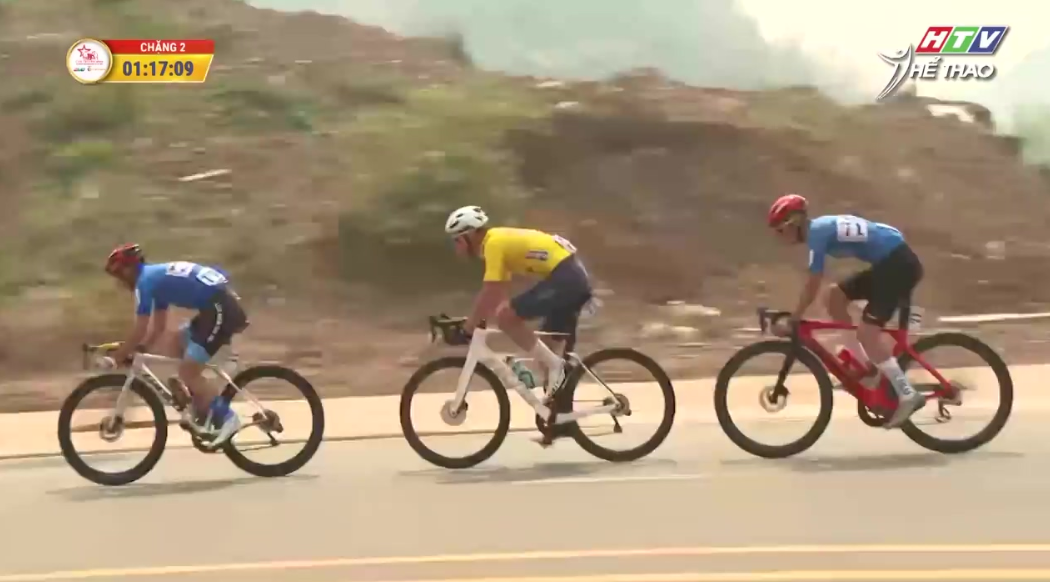
\includegraphics[width=16.5mm]{image3.png}};
  \node[draw=aicgray!70, line width=0.5pt, fill=white, inner sep=0.55mm]
    (video-front) at (0.45,2.06) {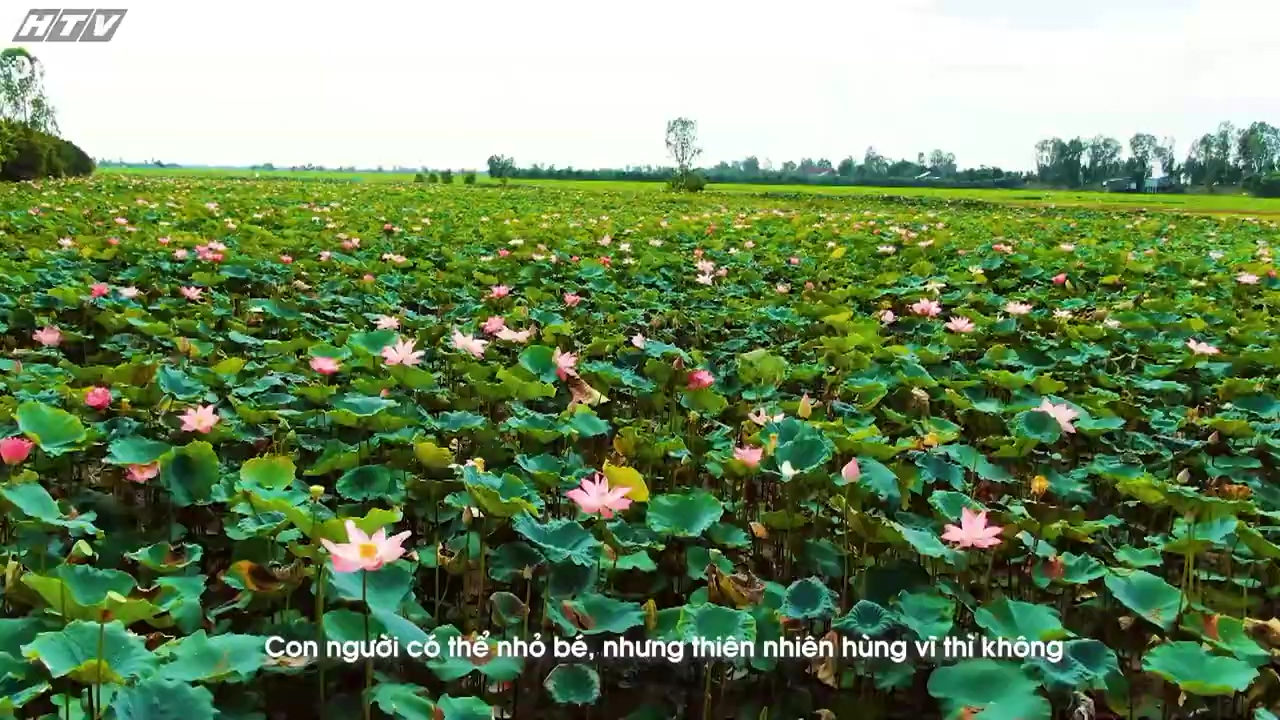
\includegraphics[width=16.5mm]{image4.png}};
  \node[font=\sffamily\scriptsize, align=center] (video-label) at (0,1.08)
    {\textbf{BTC video corpus}\\raw MP4};
  \begin{scope}[on background layer]
    \node[sourcecard, fit=(video-back)(video-mid)(video-front)(video-label)]
      (videos) {};
  \end{scope}

  \node[build] (extract) at (4.05,1.83) {\textbf{Adaptive keyframes}\\shot + saliency\\stability + coverage de-dup};
  \node[build] (registry) at (8.10,1.83) {\textbf{Frame-time registry}\\map CSV + keyframe identity\\\texttt{frame\_idx + pts\_time}};
  \node[sparse] (eskf) at (12.20,1.83) {\textbf{Elastic keyframe map}\\identity + timing};

  \node[module] (pe) at (12.20,0.48) {\textbf{PE-Core-G14}\\image embeddings};
  \node[vector] (mpe) at (16.50,0.48) {\textbf{Milvus}\\image PE vectors};

  \node[module] (ocr) at (12.20,-0.43) {\textbf{HunyuanOCR}\\spotting + cleanup};
  \node[sparse] (esocr) at (16.50,-0.43) {\textbf{Elastic}\\OCR text boxes};

  \node[optional] (caption) at (12.20,-1.34) {\textbf{NVILA captions}\\optional A1 + A2 fields};
  \node[artifact] (escap) at (16.50,-1.34) {\textbf{Caption artifact}\\JSONL + facets};

  \node[optional] (objects) at (12.20,-2.25) {\textbf{Open-vocab objects}\\optional YOLOE / GDINO};
  \node[artifact] (esobj) at (16.50,-2.25) {\textbf{Object artifact}\\JSONB + crop vectors};

  \node[build, fill=aicred!5] (decode) at (8.10,-3.64) {\textbf{Audio preparation}\\16 kHz decode + windows};
  \node[audiomodule] (speech) at (12.20,-3.18) {\textbf{PhoWhisper}\\WhisperX alignment};
  \node[sparse] (essp) at (16.50,-3.18) {\textbf{Elastic}\\speech segments};

  \node[audiomodule] (audio) at (12.20,-4.09) {\textbf{GLAP + CED}\\audio event captions};
  \node[vector] (esaud) at (16.50,-4.09) {\textbf{Elastic + Milvus}\\audio metadata + GLAP};

  \draw[flow] (videos.east) -- (extract.west);
  \draw[flow] (extract.east) -- (registry.west);

  \coordinate (registry-fork) at (10.10,1.83);
  \draw[bus] (registry.east) -- (registry-fork);
  \draw[flow] (registry-fork) -- (eskf.west);
  \draw[flow] (registry-fork) |- (pe.west);
  \draw[flow] (registry-fork) |- (ocr.west);
  \draw[flow] (registry-fork) |- (caption.west);
  \draw[flow] (registry-fork) |- (objects.west);
  \node[buslabel, rotate=90] at (9.97,-0.20) {keyframe registry};

  \draw[flow] (videos.south) |- (decode.west);
  \coordinate (audio-fork) at (10.10,-3.64);
  \draw[bus] (decode.east) -- (audio-fork);
  \draw[flow] (audio-fork) |- (speech.west);
  \draw[flow] (audio-fork) |- (audio.west);

  \draw[flow] (pe) -- (mpe);
  \draw[flow] (ocr) -- (esocr);
  \draw[flow] (caption) -- (escap);
  \draw[flow] (objects) -- (esobj);
  \draw[flow] (speech) -- (essp);
  \draw[flow] (audio) -- (esaud);
\end{tikzpicture}
}
\caption{Offline indexing and enrichment pipeline. The system extracts its own
representative keyframes from BTC videos, maps every extracted frame to
\submitpair{}, uploads sparse text/temporal metadata to Elastic, and uploads
dense image/audio vectors to Milvus. Caption and object branches share the same
identity registry and are optional offline enrichment extensions.}
\label{fig:offline-indexing}
\end{figure*}

\subsection{Keyframe Identity and Temporal Mapping}

The identity layer is a core contribution because many extraction artifacts use
environment-dependent paths. For example, OCR records may contain absolute
Kaggle paths, while PE embeddings are keyed by dataset-relative paths. These
paths are useful for provenance but unsafe for routing. \sys{} normalizes every
public frame as:
\[
  \sid = \texttt{C/V/N},
\]
where $C$ is the submit category, $V$ is the video id, and $N$ is the three-digit
ordinal assigned by the extraction pipeline. The L26 shard variants are normalized to category L26 for
display and submission. Internally, joins use \sid{} or the pair
(\vid{}, \kfn{}). The keyframe map stores \ptstime{}, FPS, and \fid{} for every
extracted keyframe and is used to map OCR frames, speech segments, audio windows, video
timeline entries, and submissions.

The media URL contract mirrors the same identity:
\[
\begin{split}
\text{keyframe: }&\texttt{B/Keyframes/Keyframes\_C/V/N.jpg},\\
\text{video: }&\texttt{B/Videos/Videos\_C/V.mp4},
\end{split}
\]
where $B$ is \texttt{MEDIA\_BASE\_URL} and $C=\texttt{group\_from\_video\_id}(V)$.

Table~\ref{tab:contracts} summarizes the canonical fields used to connect all
modalities to retrieval, media display, and submission.

\begin{table}[!t]
\centering
\caption{Core identity and join fields.}
\label{tab:contracts}
\scriptsize
\setlength{\tabcolsep}{2pt}
\begin{tabularx}{\columnwidth}{@{}>{\raggedright\arraybackslash}p{0.30\columnwidth}X>{\raggedright\arraybackslash}p{0.24\columnwidth}@{}}
\toprule
Field & Meaning & Used by \\
\midrule
\sid & Public frame id, \texttt{category/video/frame}; also \texttt{image\_id} & all result frames, keyframe map, OCR, Milvus image \\
\vid & Video stem, e.g., \texttt{K01\_V001} & grouping, media URL, timeline, submit \\
\kfn & Extracted keyframe ordinal, e.g., 1 for \texttt{001.jpg} & media URL, timeline \\
\fid & Absolute video frame index & KIS/QA/V-KIS/TRAKE result \\
\ptstime & Presentation timestamp in seconds & video seek, timeline, TRAKE order \\
\texttt{window\_id} & Audio-window primary key & Elastic audio $\leftrightarrow$ Milvus GLAP join \\
\texttt{segment\_id} & Speech segment primary key & Elastic speech \\
\bottomrule
\end{tabularx}
\end{table}

\subsection{Adaptive Keyframe Extraction}

Adaptive keyframe extraction is the first offline stage of \sys{}, not merely
an auxiliary analysis branch. The searchable image set, OCR frames, PE visual
embeddings, visual captions, and object detections are built on the
representative frames produced by this extractor. The extractor enforces the
same evidence contract as the online system: every extracted frame preserves
\vid{}, \fid{}, \ptstime{}, FPS, and keyframe ordinal so it can be displayed,
searched, and submitted without relying on environment-specific paths.

The extractor first partitions a video into shots with a three-level fallback
stack. TransNetV2 \cite{soucek2020transnetv2} is the preferred detector when its
weights are available. If it fails, PySceneDetect-style content differences are
used; if that also fails, the pipeline computes HSV histogram change at a low
sampling rate and marks large Bhattacharyya-distance jumps as cuts. Shots shorter
than 0.6 seconds are merged into a neighbor, including the first shot, to avoid
pathological fragments and transition frames.

Within each shot, sampling is driven by an event-saliency signal
\begin{equation}
S(t)=\mathrm{ReLU}\left(\alpha \Delta_v(t)+\beta \Delta_a(t)-\epsilon\right),
\label{eq:saliency}
\end{equation}
where $\Delta_v(t)$ is a low-resolution HSV visual-change score and
$\Delta_a(t)$ is the magnitude of the derivative of 100 ms audio RMS energy.
Both signals are normalized per shot by a high percentile so a quiet interview
and a visually dynamic outdoor report are compared against their own local
background. If audio extraction fails or the video has no usable audio stream,
the pipeline sets $\beta=0$ and continues with visual saliency only.

The candidate set is the union of a background grid and event-focused samples.
For short shots, the grid keeps one to five fractional positions; for shots
longer than 20 seconds, it samples at a configurable candidate FPS. Event samples
are added around local maxima of $S(t)$ within a 0.25 second window. A small
boundary margin removes frames close to shot transitions, and a per-shot cap of
40 candidates keeps GPU encoding predictable.

Candidate frames are decoded by linear traversal rather than random seeking:
the video reader calls \texttt{grab()} for most frames and \texttt{retrieve()}
only for selected indices. This matters for compressed MP4 files because random
seeks may force repeated decoding from nearby I-frames. Each candidate receives
a stability score
\begin{equation}
q(f)=0.50 q_{\mathrm{sharp}}(f)+0.30 q_{\mathrm{bright}}(f)+0.20 q_{\mathrm{contrast}}(f),
\end{equation}
where sharpness is derived from Laplacian variance, brightness uses a Gaussian
preference around mid-level exposure, and contrast uses grayscale standard
deviation. The score is used for tie-breaking, not as a hard deletion rule.

Visual features are encoded with PE-Core-G14-448
\cite{bolya2025perceptionencoder} when available, with SigLIP
\cite{zhai2023siglip} or handcrafted HSV/edge features as fallbacks. The system
runs one model copy per GPU in Kaggle T4x2 sessions and L2-normalizes all
vectors. Per-shot DBSCAN \cite{ester1996dbscan} over cosine distance selects
representative clusters without predefining the number of keyframes. For a
cluster, the selected frame maximizes
\begin{equation}
0.70 \langle e_i,\bar{e}_C\rangle + 0.30 q(f_i),
\end{equation}
combining representativeness and stability. Stable DBSCAN noise points are kept
only when they are sufficiently dissimilar to representatives already selected
for the shot.

The final video-level de-duplication uses temporally decayed coverage:
\begin{equation}
\mathrm{cov}(f,K)=\max_{k\in K}
\cos(e_f,e_k)\exp\left(-\frac{|t_f-t_k|}{\tau}\right).
\label{eq:coverage}
\end{equation}
Frame $f$ is kept when $\mathrm{cov}(f,K)<0.85$ with $\tau=60$ seconds. This
rule suppresses near duplicates inside the same event while preserving visually
similar scenes that recur minutes apart. The extractor writes
\texttt{keyframes/}, \texttt{map-keyframes/}, and \texttt{embeddings/} artifacts
with \vid{}, \fid{}, \ptstime{}, shot id, and feature-row provenance.

\begin{algorithm}[!t]
\caption{Adaptive representative keyframe extraction}
\label{alg:keyframe-extract}
\footnotesize
\begin{algorithmic}[1]
\Require Video $V$, configuration $\Theta$
\Ensure Keyframes, map CSV, and feature rows
\State $shots \gets$ TransNetV2$(V)$ if available
\If{$shots$ invalid}
  \State $shots \gets$ content-based shot detection$(V)$
\EndIf
\If{$shots$ invalid}
  \State $shots \gets$ HSV histogram cuts$(V)$
\EndIf
\State Merge shots shorter than $\Theta.minShotSec$
\ForAll{shot $s$ in $shots$}
  \State Compute low-resolution visual deltas $\Delta_v(t)$
  \State Compute audio RMS derivative $\Delta_a(t)$ if audio exists
  \State Normalize $\Delta_v,\Delta_a$ per shot
  \State $S(t) \gets \mathrm{ReLU}(\alpha\Delta_v(t)+\beta\Delta_a(t)-\epsilon)$
  \State $C \gets$ background grid samples for $s$
  \State $C \gets C \cup$ samples near local maxima of $S(t)$
  \State Remove candidates inside transition boundary margin
  \State Limit $C$ to $\Theta.maxCandidatesPerShot$
  \State Decode candidate frames by linear \texttt{grab}/\texttt{retrieve}
  \State Compute stability $q(f)$ for every $f\in C$
  \State Encode candidate embeddings $e_f$ and L2-normalize
  \State Cluster embeddings with per-shot DBSCAN
  \State Select one stable representative per cluster
  \State Keep stable DBSCAN-noise frames only if visually distinct
\EndFor
\State Sort representatives by stability and apply temporally decayed coverage
\State Write \texttt{keyframes/}, \texttt{map-keyframes/}, \texttt{embeddings/}
\end{algorithmic}
\end{algorithm}

\subsection{Structured Visual Captioning}

Structured visual captioning is an optional offline enrichment extension over
the extracted keyframe registry; the core image, OCR, speech, and audio
retrieval paths do not depend on it. When enabled, it adds filterable scene
facets and searchable descriptions without changing frame identity. The
notebook implementation uses NVILA-Lite-2B \cite{liu2024nvila}, which fits on a
single T4 and can shard the corpus by video-prefix range. It writes a resumable
\texttt{captions.jsonl} artifact and skips completed \field{keyframe_id} values
on reruns.

The captioner runs two passes. Pass A1 labels one keyframe with a strict JSON
schema. \textbf{Hard facets} are \field{scene_type}, \field{location_type},
\field{time_of_day}, \field{weather}, \field{camera_shot}, and
\field{num_people}. Their values come from small controlled vocabularies so they
can be used as filters. \textbf{Soft descriptions} are \field{event_type},
\field{people_roles}, \field{people_description}, \field{key_objects},
\field{dominant_colors}, \field{distinctive_detail}, \field{summary}, and
\field{text_on_screen}. Parser code extracts the first valid JSON object,
coerces out-of-vocabulary hard values to \texttt{unknown} (or \texttt{0} for
people count), and records uncertain values for later auditing.

Pass A2 optionally feeds a short neighborhood around the keyframe to identify
motion or action tags such as speaking, walking, vehicle moving, fire spreading,
or static. This pass captures evidence that a single frame cannot express. Near
duplicates are grouped by difference hash, so repeated frames can inherit the
representative's metadata rather than spending VLM budget repeatedly.

The optional caption index is split by retrieval use. For V-KIS, the prompt
clip is observed by an operator and on-screen text may be removed, so
\field{text_on_screen} is excluded from V-KIS soft matching and retained for
T-KIS/QA. The text-independent fields are concatenated into a caption string and
embedded with a multilingual sentence encoder for text-to-caption search. A
separate optional SigLIP image-vector index supports text-to-image search from
operator descriptions. The facet table supports hard filtering before ranking,
while caption vectors support soft semantic retrieval.

\begin{algorithm}[!t]
\caption{Structured visual captioning extension}
\label{alg:captioning}
\footnotesize
\begin{algorithmic}[1]
\Require Extracted keyframe records $\mathcal{K}$
\Ensure Caption JSONL and optional caption/image vectors
\State Load completed \texttt{keyframe\_id}s from existing JSONL
\ForAll{video shard $V$}
  \State Read ordered keyframe refs from \texttt{map-keyframes}
  \State Group near duplicates by difference hash
  \ForAll{keyframe $k$ not yet completed}
    \State Run A1 single-image prompt with strict JSON schema
    \State Extract JSON; coerce hard fields to allowed vocabularies
    \If{A2 enabled}
      \State Run A2 neighborhood prompt for \texttt{action\_motion}
    \EndIf
    \State Merge identity, A1/A2 fields, dedup group, and model version
    \State Append one JSONL record and flush
  \EndFor
\EndFor
\State Build facets and optional semantic embedding indices
\end{algorithmic}
\end{algorithm}

\subsection{Open-vocabulary Object Detection}

Closed-set detectors trained on COCO-like labels miss broadcast-specific
entities: Vietnamese TV logos, lower-third graphics, local signs, uniforms,
anchors, emergency vehicles, ceremonial objects, and rare news objects. The
project therefore treats object detection as an optional zero-shot,
no-fine-tuning enrichment branch over keyframes, not as a dependency of the
core hybrid retriever. Its evidence record contains
\texttt{label}, \texttt{bbox}, \texttt{conf}, \texttt{source},
\texttt{color}, \texttt{grid\_cell}, optional \texttt{crop\_emb\_id}, and
per-label counts.

The full design uses an ensemble. YOLOE \cite{wang2025yoloe} provides fast
open-vocabulary bulk tagging; Grounding DINO \cite{liu2024groundingdino} or
MM-Grounding-DINO
provides prompt-specific grounding for rarer concepts; a Qwen-style VLM
grounding pass is reserved for dense or ambiguous cases such as counting
crowds. The Kaggle notebook defaults to YOLOE-only for throughput and exposes an
A/B cell that estimates the additional boxes and labels contributed by the
ensemble before deciding whether the extra runtime is worth it.

Prompt vocabulary is genre-conditional. A base vocabulary covers common
objects such as person, crowd, text on screen, logo, microphone, sign, table,
car, and motorbike. Genre-specific vocabularies are selected from the video
prefix: news, cycling, lion dance, exam, cooking, culture, Mekong, and positive
shorts use different concept lists. This reduces detector noise and avoids
wasting prompt budget on objects that are implausible for a program genre.

When multiple detectors are enabled, overlapping boxes are fused with weighted
box fusion \cite{solovyev2021wbf}. For boxes with the same label and
intersection-over-union above a threshold, the fused box is
\begin{equation}
b^\ast=\frac{\sum_i s_i w_i b_i}{\sum_i s_i w_i},
\end{equation}
where $s_i$ is detector confidence and $w_i$ is a model weight. This preserves
agreement across detectors instead of discarding boxes as non-maximum
suppression would. Boxes seen by only one detector may be retained with lower
confidence for recall.

Each detection is enriched with attributes that are cheap but useful for
compositional queries. The bbox center is mapped to a 7x7 spatial grid for
phrases such as ``upper left'' or ``right side''. Dominant color is computed by
cropping the box and quantizing to a 16-color palette. Counts are stored per
label, with dense scenes optionally delegated to a VLM counter. High-confidence
crops are encoded with DINOv2-style crop embeddings \cite{oquab2023dinov2} for
instance search, such as finding the same logo or vehicle shape again. Metadata
can be stored as JSONB-style records, while crop embeddings enter a separate
Milvus collection.

Because the project has no exhaustive object labels, validation is weakly
supervised. The branch compares overlapping labels against BTC-provided object
metadata where available, runs manual spot checks on random keyframes,
monitors cross-model consistency, and renders bbox overlays for qualitative
vocabulary and threshold tuning. The objective is not to claim mAP, but to
choose usable confidence thresholds and genre vocabularies.

\begin{algorithm}[!t]
\caption{Zero-shot object enrichment}
\label{alg:object-enrich}
\footnotesize
\begin{algorithmic}[1]
\Require Extracted keyframes $\mathcal{K}$, genre vocabularies
\Ensure Detection JSONL and optional crop embeddings
\ForAll{keyframe $k$}
  \State Infer genre and build the allowed concept list
  \State Run YOLOE open-vocabulary detection
  \If{ensemble enabled}
    \State Run Grounding-DINO on concept chunks
    \State Fuse same-label overlaps with WBF
  \EndIf
  \ForAll{detection $d$}
    \State Store label, confidence, source list, and bbox
    \State Derive 7x7 grid cell and dominant crop color
    \If{$conf(d)\geq \Theta.cropConf$}
      \State Encode crop and store \texttt{crop\_emb\_id}
    \EndIf
  \EndFor
  \State Store label counts and append the JSONL record
\EndFor
\State Validate with weak references and rendered bbox audits
\end{algorithmic}
\end{algorithm}

\subsection{Visual Embedding Index}

The visual channel uses PE-Core-G14-448 embeddings
\cite{bolya2025perceptionencoder}, following the general contrastive text-image
retrieval paradigm popularized by CLIP \cite{radford2021clip}. The image collection
\texttt{aic26\_image\_peg14\_v1} contains 382,299 vectors of dimension 1280 and
uses cosine similarity. Each Milvus entity stores the canonical id, category,
video id, keyframe number, provenance path, and vector. At query time, a PE text
encoder endpoint converts the English visual query into a vector, and Milvus
returns ranked keyframes. When query expansion is enabled, several compact
English visual variants are encoded and searched independently; results are
merged by maximum cosine score per frame before entering the channel-fusion
stage.

\subsection{OCR Index}

OCR is extracted with HunyuanOCR \cite{hunyuanocr2025} in text-spotting mode. The pipeline parses model
outputs into text boxes, normalizes Unicode to NFC, creates a folded
diacritic-free representation, and writes one record per keyframe. A
post-processing step removes boxes that are pure broadcast clock, station logo,
watermark, YouTube button, single-character noise, or coordinate remnants, while
preserving text that appears inside meaningful sentences. It adds
\texttt{text\_clean}, \texttt{text\_clean\_fold}, \texttt{clock}, and
\texttt{hour}. The Elastic OCR index contains 382,299 records. The retrieval
adapter searches \texttt{text\_clean}, \texttt{text\_nfc}, and fuzzy folded text,
with optional hour and clock filters. Empty OCR queries never fall through to
match-all.

\subsection{Speech Transcript Index}

Speech extraction begins by decoding each MP4 to 16 kHz mono audio.
\mbox{PhoWhisper-large} \cite{le2024phowhisper} performs Vietnamese ASR through CTranslate2, and
WhisperX forced alignment assigns word-level timestamps and alignment scores
\cite{bain2023whisperx}. A faster-Whisper path remains as a
fallback when the aligner is unavailable. Extraction is checkpointed per video:
each \texttt{.speech.json} file stores the transcript text, segment start/end,
word timestamps, word scores, and backend-specific confidence metadata.

Index construction, detailed in Algorithm~\ref{alg:speech-index}, deliberately
keeps uncertain segments so thresholds can be changed without rerunning ASR.
The mapper creates a stable \field{segment_id}, computes
\field{avg_word_score}, and assigns confidence as low below $0.40$, mid in
$[0.40,0.50)$, high at or above $0.50$, or missing. It also labels each segment
as intro, preview, or body. The segment start, center, and end times are mapped
independently to the nearest extracted keyframes; the center mapping becomes the
canonical \sid{} while all three anchors remain available for temporal
inspection and TRAKE.

The Elastic index contains 48,819 segments across 1,478 videos. Vietnamese text
queries use full-text and boosted phrase matching. Before channel fusion, the
Elastic score is multiplied by confidence factors
$\{1.0,0.75,0.25,0.5\}$ for high, mid, low, and missing confidence, and role
factors $\{1.0,0.7,0.6\}$ for body, intro, and preview. Thus weak or promotional
segments remain retrievable but are less likely to become incorrect temporal
anchors. Fig.~\ref{fig:speech-audio-indexing} illustrates the complete mapping
from MP4 audio to the searchable speech record.

\begin{algorithm}[!t]
\caption{Speech transcript indexing}
\label{alg:speech-index}
\footnotesize
\begin{algorithmic}[1]
\Require Video $V$, extracted-keyframe registry $K$
\Ensure Mapped speech-segment records for Elastic
\State $x \gets$ decode $V$ as 16 kHz mono audio
\State $S \gets$ PhoWhisper-ASR$(x)$
\State $S \gets$ WhisperX-Align$(x,S)$ if available
\ForAll{segment $s\in S$}
  \State Normalize text and retain word timestamps/scores
  \State Assign confidence bucket and temporal role
  \State $k_s \gets \Call{NearestKeyframe}{K,V,s.start}$
  \State $k_c \gets \Call{NearestKeyframe}{K,V,s.center}$
  \State $k_e \gets \Call{NearestKeyframe}{K,V,s.end}$
  \State Build stable \texttt{segment\_id} from video and span
  \State Set canonical submit id from $k_c$; retain $k_s,k_c,k_e$
  \State Append segment without hard-deleting low confidence
\EndFor
\State Bulk-upload records to the Elastic speech index
\end{algorithmic}
\end{algorithm}

\subsection{Audio Event Index}

The non-speech audio branch targets cues that ASR cannot represent, such as
music, applause, bells, engines, animal sounds, and kitchen events. After the
same 16 kHz conversion, each video is divided into five-second windows with a
2.5-second hop. Every window receives a normalized 1024-dimensional GLAP
embedding \cite{dinkel2025glap} and the top five CED tags
\cite{dinkel2023ced} with scores. A MiDashengLM caption
\cite{dinkel2025midashenglm} is generated only when the highest-scoring tag passes the
non-speech gate, limiting caption cost and preventing narration from dominating
the caption branch. The extractor writes one \texttt{.audio.json} record per
window and one row in a float16 \texttt{.glap.npy} matrix, connected by
\field{glap_idx}.

Algorithm~\ref{alg:audio-index} describes index construction. The mapper creates
a stable \field{window_id}, maps window start, center, and end to the frame-time
registry, and derives quality fields before upload. Captions are classified as
useful, generic, Vietnamese-ASR leakage, or absent. CED labels known to be noisy
on Vietnamese narration, especially \emph{Speech synthesizer} and
\emph{Mantra}, set stoplist flags rather than modifying the raw extraction
artifact. This separation makes the extraction reproducible while allowing the
retrieval policy to evolve.

The resulting corpus contains 466,996 windows and 35,222 caption records.
Elastic stores timing, tags, scores, captions, quality flags, and keyframe
anchors; Milvus stores GLAP vectors keyed by the same \field{window_id}. Online
retrieval therefore has two complementary ranked lists: Elastic matches exact
labels and caption text, while GLAP matches a semantic sound query in vector
space. A stoplisted top-1 label is dropped, weaker quality signals are demoted,
and the surviving Elastic and GLAP lists are merged by rank-RRF with $k=30$
before entering global multi-channel fusion.

\begin{algorithm}[!t]
\caption{Audio-event index construction}
\label{alg:audio-index}
\footnotesize
\begin{algorithmic}[1]
\Require Video $V$, extracted-keyframe registry $K$
\Ensure Elastic audio records and Milvus GLAP vectors
\State $x \gets$ decode $V$ as 16 kHz mono audio
\State $W \gets$ five-second windows with 2.5-second hop
\ForAll{window $w_i\in W$}
  \State $g_i \gets$ L2-normalized GLAP embedding of $w_i$
  \State $T_i \gets$ CED top-5 labels and scores for $w_i$
  \If{top-1 label is non-speech and passes caption gate}
    \State $p_i \gets$ MiDashengLM caption$(w_i)$
  \Else
    \State $p_i \gets \varnothing$
  \EndIf
  \State Classify caption quality and mark stoplist hits
  \State Map start, center, and end to nearest keyframes in $K$
  \State Build \texttt{window\_id}; append metadata with \texttt{glap\_idx}$=i$
  \State Store $g_i$ as row $i$ of the video GLAP shard
\EndFor
\State Upload metadata to Elastic and vectors to Milvus by window id
\end{algorithmic}
\end{algorithm}

\begin{figure*}[t]
\centering
\resizebox{0.98\textwidth}{!}{%
\begin{tikzpicture}[
  stage/.style={draw=aicgray!78, line width=0.65pt, rounded corners=2pt,
    align=center, font=\sffamily\scriptsize, minimum height=10mm,
    text width=22mm, fill=white},
  shared/.style={stage, fill=aicblue!6},
  speechpipe/.style={stage, fill=aicgreen!6},
  audiopipe/.style={stage, fill=aicorange!6},
  mapper/.style={stage, fill=aiccyan!6, text width=27mm, minimum height=21mm},
  store/.style={stage, fill=aicgray!5, text width=29mm, minimum height=13mm},
  flow/.style={-{Latex[length=1.9mm, width=1.25mm]}, draw=aicgray!90,
    line width=0.75pt},
  bus/.style={draw=aicgray!78, line width=0.7pt},
  phase/.style={font=\sffamily\scriptsize\bfseries, text=aicgray,
    anchor=west}
]
  \node[phase] at (-1.30,2.50) {SHARED AUDIO INPUT};
  \draw[aiccyan!70, line width=0.8pt] (-1.30,2.23) -- (4.55,2.23);
  \node[phase] at (5.00,2.50) {PARALLEL EVIDENCE EXTRACTION};
  \draw[aicgreen!65, line width=0.8pt] (5.00,2.23) -- (13.65,2.23);
  \node[phase] at (14.10,2.50) {TEMPORAL MAPPING AND STORAGE};
  \draw[aicorange!65, line width=0.8pt] (14.10,2.23) -- (20.80,2.23);

  \node[shared] (mp4) at (0,0) {BTC video\\raw MP4};
  \node[shared] (wav) at (3.20,0) {FFmpeg decode\\16 kHz mono};

  \node[speechpipe] (asr) at (6.25,1.05) {\textbf{PhoWhisper}\\segment ASR};
  \node[speechpipe] (align) at (9.25,1.05) {\textbf{WhisperX}\\word alignment};
  \node[speechpipe] (sqc) at (12.25,1.05) {Confidence bucket\\segment role};

  \node[audiopipe] (windows) at (6.25,-1.05) {5 s windows\\2.5 s hop};
  \node[audiopipe] (features) at (9.25,-1.05) {\textbf{GLAP + CED}\\vector + top-5 tags};
  \node[audiopipe] (gate) at (12.25,-1.05) {Caption gate\\quality + stoplist};

  \node[mapper] (mapping) at (15.65,0) {\textbf{Frame-time registry}\\nearest keyframes at\\start / center / end};
  \node[store] (sstore) at (19.45,1.05) {
    
\includegraphics[height=4.0mm]{elasticlogo.png}\\[-0.3mm]
    \textbf{Elastic speech index}\\text + temporal anchors};
  \node[store] (astore) at (19.45,-1.05) {
    
\includegraphics[height=3.8mm]{elasticlogo.png}\hspace{1.5mm}
    
\includegraphics[height=3.8mm]{milvuslogo.png}\\[-0.3mm]
    \textbf{Audio indices}\\metadata + GLAP vectors};

  \draw[flow] (mp4) -- (wav);
  \coordinate (decode-fork) at (4.75,0);
  \draw[bus] (wav.east) -- (decode-fork);
  \draw[flow] (decode-fork) |- (asr.west);
  \draw[flow] (decode-fork) |- (windows.west);

  \draw[flow] (asr) -- (align);
  \draw[flow] (align) -- (sqc);
  \draw[flow] (sqc.east) -- ([yshift=4.5mm]mapping.west);
  \draw[flow] ([yshift=4.5mm]mapping.east) -- (sstore.west);

  \draw[flow] (windows) -- (features);
  \draw[flow] (features) -- (gate);
  \draw[flow] (gate.east) -- ([yshift=-4.5mm]mapping.west);
  \draw[flow] ([yshift=-4.5mm]mapping.east) -- (astore.west);
\end{tikzpicture}
}
\caption{Speech and audio-event index construction. Both branches share the
decoded waveform and frame-time registry but preserve different evidence:
aligned Vietnamese transcript segments in Elastic, and audio tags/captions in
Elastic plus GLAP vectors in Milvus. Mapping each time span at its start, center,
and end keeps retrieval evidence connected to inspectable and submit-safe
keyframes.}
\label{fig:speech-audio-indexing}
\end{figure*}

\section{Online Query Processing and Retrieval}

\subsection{Query Understanding}

The parser produces a structured routing object with task type, channel enable
flags, channel weights, channel-specific query strings, filters, TRAKE events,
QA settings, and UI hints. There are two parser paths.

\textbf{Heuristic parser.} The deterministic parser detects OCR-likely queries
from digits, visible-text cues, quotes, or clock patterns; speech-likely queries
from verbs such as \emph{speak}, \emph{announce}, or \emph{interview}; audio
queries from non-speech sound words; and TRAKE queries from explicit event
markers or chronological connectors. It enables image search by default, adds
OCR/speech/audio only when cues are present, and guarantees that at least one
retrieval channel remains active.

\textbf{LLM parser.} When enabled, the backend calls an OpenAI-compatible NVIDIA
NIM endpoint. The LLM returns JSON under a strict schema and may generate compact
English visual paraphrases for dense image search. If the LLM is unavailable or
produces invalid JSON after retry, the system falls back to heuristics. When the
LLM is disabled, Vietnamese queries are translated to English for the PE visual
channel; OCR and speech remain in Vietnamese. This translation is a best-effort,
external machine-translation service in the implementation; if it fails or the
input already appears to be English, the original string is used unchanged. No
online translation is used for the reported TKIS evaluation.

\begin{algorithm}[!t]
\caption{Heuristic query routing}
\label{alg:routing}
\footnotesize
\begin{algorithmic}[1]
\Require Query $q$, task hint $h$, previous hints $P$
\State $x \gets$ concatenate$(P,q)$
\State Enable image channel with visual query $x$
\If{$x$ contains digits, quotes, clock, or visible-text words}
  \State Enable OCR with exact, folded, and time filters
\EndIf
\If{$x$ contains speech verbs}
  \State Enable speech with Vietnamese query $x$
\EndIf
\If{$x$ contains non-speech sound words}
  \State Enable audio with English sound labels if known
\EndIf
\If{$h$ is TRAKE or $x$ has event connectors}
  \State Split $q$ into ordered events $E_1,\ldots,E_n$
  \State Create per-event visual/OCR/speech/audio fields
\EndIf
\State Apply manual channel overrides
\If{all channels disabled}
  \State Re-enable image channel
\EndIf
\State Return routing JSON
\end{algorithmic}
\end{algorithm}

\subsection{Multi-channel Retrieval}

Fig.~\ref{fig:online-retrieval} details online retrieval. Each enabled channel
returns ranked \texttt{ChannelHit} objects containing \sid{}, \vid{}, \kfn{},
rank, raw score, timestamp if available, and evidence.

\begin{figure*}[t]
\centering
\resizebox{0.98\textwidth}{!}{%
\begin{tikzpicture}[
  stage/.style={draw=aicgray!78, line width=0.65pt, rounded corners=2pt,
    align=center, font=\sffamily\scriptsize, minimum height=11mm,
    text width=22mm, fill=white},
  querybox/.style={stage, fill=aicblue!6},
  parserbox/.style={stage, fill=aiccyan!6, text width=25mm},
  retrieval/.style={stage, text width=24mm, minimum height=10mm},
  fusion/.style={stage, fill=aicgreen!6, text width=25mm, minimum height=15mm},
  grouping/.style={stage, fill=aicorange!6, text width=26mm, minimum height=15mm},
  interface/.style={stage, fill=aicblue!6, text width=26mm, minimum height=15mm},
  media/.style={stage, fill=aicgray!5, text width=26mm, minimum height=13mm},
  flow/.style={-{Latex[length=1.9mm, width=1.25mm]}, draw=aicgray!90,
    line width=0.75pt},
  feedback/.style={-{Latex[length=1.8mm, width=1.2mm]}, draw=aiccyan!90,
    line width=0.7pt},
  bus/.style={draw=aicgray!78, line width=0.7pt},
  phase/.style={font=\sffamily\scriptsize\bfseries, text=aicgray,
    anchor=west},
  flowlabel/.style={font=\sffamily\tiny, text=aicgray, fill=white,
    inner sep=1pt}
]
  \node[phase] at (-1.25,2.75) {QUERY PLANNING};
  \draw[aiccyan!70, line width=0.8pt] (-1.25,2.48) -- (4.70,2.48);
  \node[phase] at (5.10,2.75) {PARALLEL RETRIEVAL};
  \draw[aicgreen!65, line width=0.8pt] (5.10,2.48) -- (8.70,2.48);
  \node[phase] at (9.10,2.75) {FUSION, GROUPING, AND INSPECTION};
  \draw[aicorange!65, line width=0.8pt] (9.10,2.48) -- (18.85,2.48);

  \node[querybox] (query) at (0,0) {\textbf{User query}\\text or voice};
  \node[parserbox] (parser) at (3.15,0) {\textbf{Cue-aware parser}\\VI / EN query fields\\channel weights};

  \node[retrieval, fill=aicblue!5] (image) at (6.60,1.65) {
    
\includegraphics[height=3.2mm]{milvuslogo.png}\\[-0.2mm]
    \textbf{PE visual}\\cosine vector search};
  \node[retrieval, fill=aicorange!5] (ocr) at (6.60,0.55) {
    
\includegraphics[height=3.2mm]{elasticlogo.png}\\[-0.2mm]
    \textbf{OCR}\\BM25 + fuzzy text};
  \node[retrieval, fill=aicorange!5] (speech) at (6.60,-0.55) {
    
\includegraphics[height=3.2mm]{elasticlogo.png}\\[-0.2mm]
    \textbf{Speech}\\phrase + confidence};
  \node[retrieval, fill=aicblue!5] (audio) at (6.60,-1.65) {
    
\includegraphics[height=2.9mm]{elasticlogo.png}\hspace{1.2mm}
    
\includegraphics[height=2.9mm]{milvuslogo.png}\\[-0.2mm]
    \textbf{Audio}\\text + GLAP vectors};

  \node[fusion] (rrf) at (10.40,0) {\textbf{Weighted RRF}\\merge by canonical\\frame ID + evidence};
  \node[grouping] (group) at (13.85,0) {\textbf{Video grouping}\\timing enrichment\\ranked evidence};
  \node[interface] (ui) at (17.35,0) {\textbf{React operator UI}\\video + timeline\\submission guard};
  \node[media] (r2) at (13.85,-2.05) {
    
\includegraphics[height=3.8mm]{Cloudflare_Logo.png}\\[-0.2mm]
    \textbf{Cloudflare R2}\\keyframes + videos};

  \draw[flow] (query) -- (parser);
  \coordinate (route-fork) at (4.90,0);
  \draw[bus] (parser.east) -- (route-fork);
  \draw[flow] (route-fork) |- (image.west);
  \draw[flow] (route-fork) |- (ocr.west);
  \draw[flow] (route-fork) |- (speech.west);
  \draw[flow] (route-fork) |- (audio.west);

  \coordinate (hit-merge) at (8.55,0);
  \draw[bus] (image.east) -| (hit-merge);
  \draw[bus] (ocr.east) -| (hit-merge);
  \draw[bus] (speech.east) -| (hit-merge);
  \draw[bus] (audio.east) -| (hit-merge);
  \draw[flow] (hit-merge) -- (rrf.west);
  \draw[flow] (rrf) -- (group);
  \draw[flow] (group) -- (ui);
  \draw[flow] (r2.east) -| node[flowlabel, near end, right]{media} (ui.south);
\end{tikzpicture}
}
\caption{Online query execution. The parser creates a channel plan; channels run
in parallel; ranked lists are fused by \rrf{} and grouped for video-centric
inspection, while Cloudflare R2 supplies keyframe and video media to the UI.}
\label{fig:online-retrieval}
\end{figure*}

\textbf{Image PE.} The channel encodes English visual queries, searches Milvus,
and converts hits into frame candidates. With expansion, each paraphrase is
searched separately and only the best cosine per frame is kept.

\textbf{OCR.} The channel searches clean Vietnamese text, NFC text, and folded
fuzzy text, with optional exact phrases and clock/hour filters.

\textbf{Speech.} The channel searches ASR segments and demotes lower-confidence
or structurally less useful segments.

\textbf{Audio.} Elastic audio search ranks tag and caption matches after
stoplist/caption-quality filtering. GLAP vector hits are searched in Milvus
when the audio text encoder is available. The two audio lists are fused by a
small-$k$ rank fusion into a single audio channel list.

\subsection{Reciprocal Rank Fusion}

Given channel ranked lists $\mathcal{L}_c$, each frame $d$ receives the
reciprocal rank fusion score \cite{cormack2009rrf}
\[
  s_{\mathrm{RRF}}(d)=\sum_{c}
  \mathbb{I}[d \in \mathcal{L}_c]\frac{w_c}{k+r_c(d)+1},
\]
where $r_c(d)$ is the zero-based rank of $d$ in channel $c$, $w_c$ is the
channel weight from the parser/operator, and $k=60$ by default. Fusion is
performed over \sid{}, so evidence from multiple channels attaches to the same
canonical frame. Relevance feedback applies deterministic post-fusion edits:
positive videos receive a small boost, negative frames are dropped, and negative
videos are demoted.

\begin{algorithm}[!t]
\caption{Channel fusion and video grouping}
\label{alg:fusion}
\footnotesize
\begin{algorithmic}[1]
\Require Ranked lists $\{\mathcal{L}_c\}$, channel weights $\{w_c\}$
\State Initialize map $F$ from \sid{} to fused frame
\ForAll{channels $c$}
  \ForAll{hit $d$ at zero-based rank $r$ in $\mathcal{L}_c$}
    \State $F[d].score \mathrel{+}= w_c/(k+r+1)$
    \State Attach channel badge and evidence to $F[d]$
  \EndFor
\EndFor
\State Apply frame/video feedback edits
\State Batch-fetch missing \ptstime{}, \fid{}, and FPS
\State Group fused frames by \vid{}
\ForAll{video groups $V$}
  \State Sort frames and compute aggregate group score
  \State Mark ambiguous groups with a large temporal gap
\EndFor
\State Return video groups sorted by composite score
\end{algorithmic}
\end{algorithm}

\subsection{Video-level Grouping and Evidence Aggregation}

Fused frames are grouped by \vid{}. A video score is computed from the strongest
frame, the mean of the top frames, and temporal support around the best frame:
\[
\begin{split}
  S(V) &= 0.75 \cdot \frac{s_{\max}(V)}{s_{\max}^{global}}
       + 0.15 \cdot \frac{\mathrm{meanTop3}(V)}{s_{\max}^{global}}\\
       &\quad + 0.10 \cdot \mathrm{clusterSupport}(V).
\end{split}
\]
This coverage-aware but best-frame-dominant score prevents videos with many weak
hits from burying a video with a single strong hit. If the top timestamps within
a video are separated by a large gap, the group is marked ambiguous so the
operator knows to inspect multiple temporal clusters.
Here, $\mathrm{clusterSupport}(V)$ is the normalized local support around the
best frame: the system counts fused frames whose timestamps fall within
$\pm 30$ seconds of the highest-scoring frame, subtracts the best frame itself,
and divides by four, clipping the result to $[0,1]$. Ambiguity is marked when
the sorted timestamps of the top five frames contain a gap larger than 30
seconds. The grouping weights 0.75/0.15/0.10 are heuristic values selected for
operator-oriented ranking and were not learned from the 14-query evaluation
set.

\section{Temporal Action Retrieval for TRAKE}

\subsection{Event Decomposition}

A TRAKE query is parsed into events $E_1,\dots,E_n$. Explicit markers such as
\texttt{E1:} and \texttt{E2:} are preferred; otherwise chronological connectors
such as ``then'', ``after that'', or Vietnamese equivalents are used. Each event
receives visual, OCR, speech, and audio query fields. The default ordering rule
is strict increasing time within one video.

\subsection{Per-event Retrieval}

The TRAKE service runs the normal retrieval stack for each event independently
and concurrently, using a wider candidate pool than standard KIS. This yields
per-event frame lists $\mathcal{F}_1,\dots,\mathcal{F}_n$. Candidate frames
without timestamps are excluded from sequence assembly because the temporal
constraint cannot be evaluated.

\subsection{Dynamic Programming Sequence Assembly}

For each video, event candidates form a directed acyclic graph ordered by event
index and timestamp. An edge from candidate $u$ to candidate $v$ exists when
$u.event < v.event$ and $u.time < v.time$. The objective is to maximize event
coverage first and relevance second, represented directly as the tuple
$(\mathrm{coverage},\mathrm{relevance})$ and compared lexicographically. Thus,
adding one covered event always dominates any relevance difference among chains
with fewer covered events. The exact dynamic program over the retrieved
candidate set is shown in Algorithm~\ref{alg:trake-dp}.

\textbf{Complexity.} For one video, let $M=|N|$ be the total number of retained
event candidates. Sorting the candidates costs $O(M\log M)$. The implementation
examines every earlier candidate for each node, so the dynamic program costs
$O(M^2)$ time; the value and parent arrays require $O(M)$ memory. With $n$ events
and the deployed per-event, per-video cap $c=12$, $M\leq nc$, giving
$O(n^2c^2)$ time and $O(nc)$ memory per video. Across a set of candidate videos
$\mathcal{V}$, sequence assembly costs
$O(\sum_{V\in\mathcal{V}} M_V^2)$ after sorting. Encoder and index-search latency
belongs to per-event retrieval and is not included in this DP bound.

\begin{algorithm}[t]
\caption{TRAKE lexicographic increasing-chain DP}
\label{alg:trake-dp}
\begin{algorithmic}[1]
\Require Candidate lists $\mathcal{F}_1,\ldots,\mathcal{F}_n$
\Ensure One ordered pick per covered event
\State $N \gets$ all candidates sorted by $(event,time)$
\ForAll{$i \in 1,\ldots,|N|$}
  \State $dp[i] \gets (1, score(N_i))$
  \State $parent[i] \gets \bot$
  \ForAll{$j < i$}
    \If{$event(N_j)<event(N_i)$ and $time(N_j)<time(N_i)$}
      \State $cand \gets (dp[j].coverage + 1, dp[j].relevance + score(N_i))$
      \If{$cand >_{\mathrm{lex}} dp[i]$}
        \State $dp[i] \gets cand$
        \State $parent[i] \gets j$
      \EndIf
    \EndIf
  \EndFor
\EndFor
\State Trace back from $\arg\max_i dp[i]$
\State Return selected candidates indexed by event
\end{algorithmic}
\end{algorithm}

\begin{figure}[t]
\centering
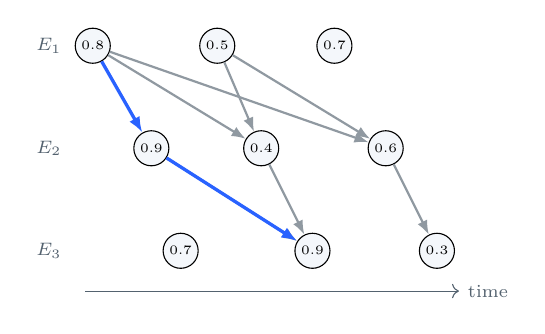
\begin{tikzpicture}[node distance=7mm and 11mm, scale=0.93, transform shape]
  \node[note] at (-0.6,2.0) {$E_1$};
  \node[note] at (-0.6,0.6) {$E_2$};
  \node[note] at (-0.6,-0.8) {$E_3$};
  \foreach \x/\y/\name/\score in {0/2.0/a/0.8,1.7/2.0/b/0.5,3.3/2.0/c/0.7,
                                  0.8/0.6/d/0.9,2.3/0.6/e/0.4,4.0/0.6/f/0.6,
                                  1.2/-0.8/g/0.7,3.0/-0.8/h/0.9,4.7/-0.8/i/0.3}
    \node[circle, draw, fill=aiclight, inner sep=1.6pt] (\name) at (\x,\y) {\tiny \score};
  \draw[faintarrow] (a) -- (e);
  \draw[faintarrow] (a) -- (f);
  \draw[faintarrow] (b) -- (e);
  \draw[faintarrow] (b) -- (f);
  \draw[faintarrow] (d) -- (h);
  \draw[faintarrow] (e) -- (h);
  \draw[faintarrow] (f) -- (i);
  \draw[arrow, very thick, draw=aicblue] (a) -- (d);
  \draw[arrow, very thick, draw=aicblue] (d) -- (h);
  \draw[->, aicgray] (-0.1,-1.35) -- (5.0,-1.35) node[right, font=\scriptsize] {time};
\end{tikzpicture}
\caption{TRAKE candidates form a DAG over event index and time. The selected
path maximizes coverage before relevance; it may skip locally high candidates
that block a better ordered chain.}
\label{fig:trake-dag}
\end{figure}

\begin{figure*}[t]
\centering
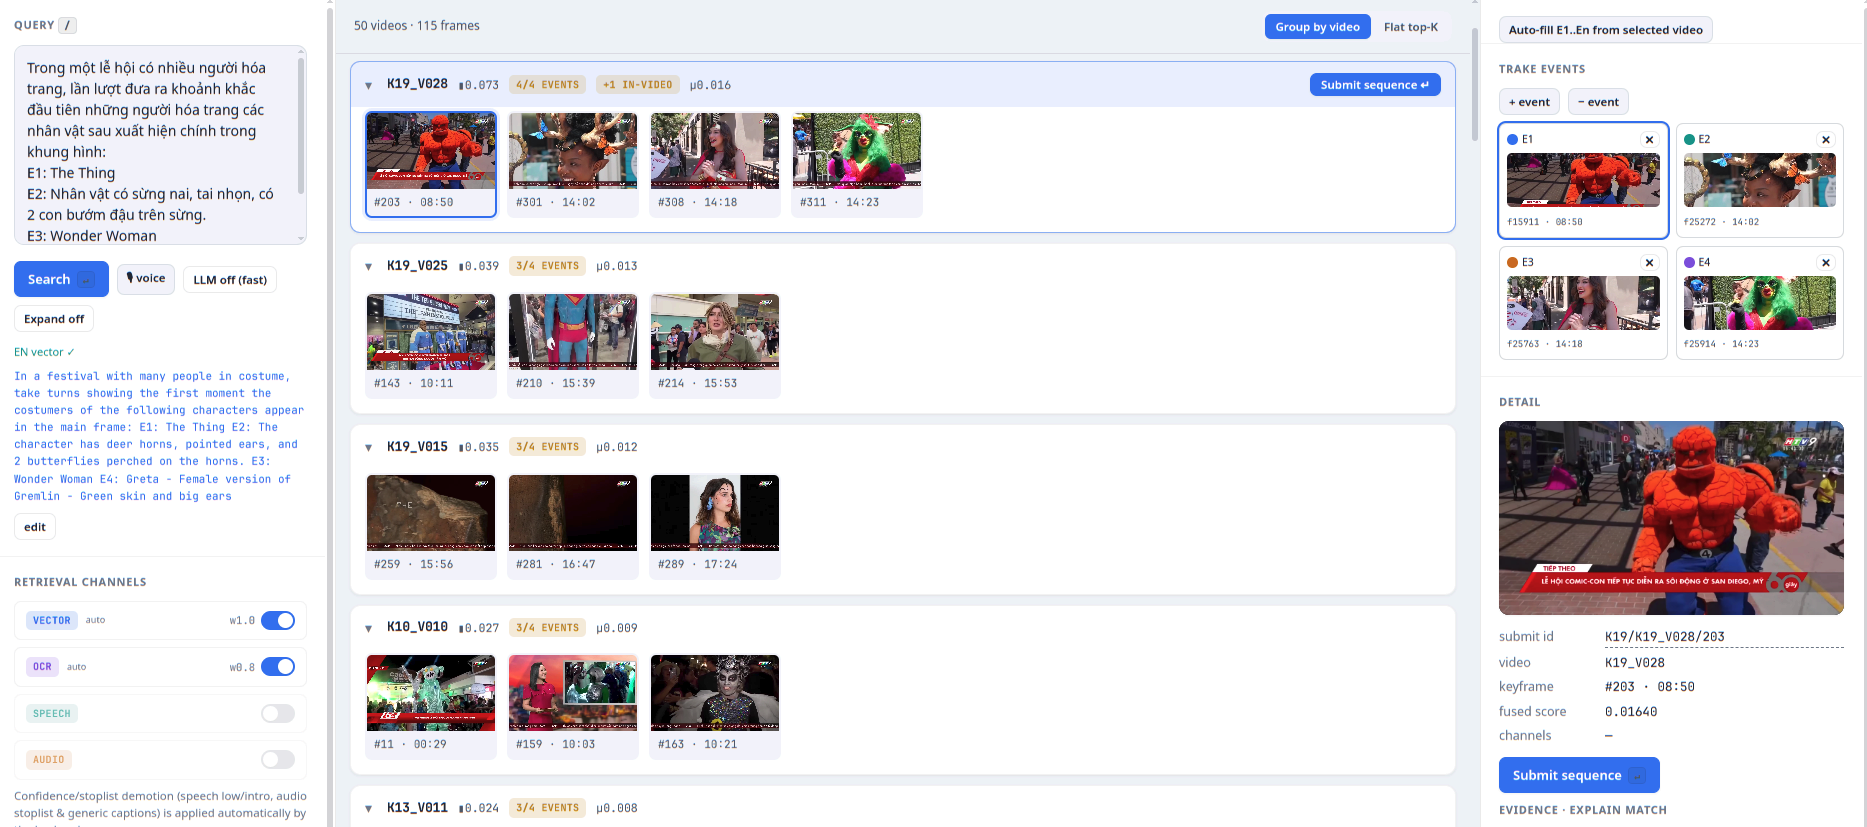
\includegraphics[width=0.98\textwidth]{trake_ui.png}
\caption{TRAKE interface for inspecting ordered event candidates. The UI keeps
event slots, candidate evidence, video context, and submit controls visible so
the operator can verify temporal order before submitting a sequence.}
\label{fig:trake-ui}
\end{figure*}

\subsection{Two-pass In-video Fill}

After pass 1, some promising videos cover only a subset of events. The service
then performs targeted in-video searches for missing events using Milvus filters
on \vid{}. A fill candidate must exceed a relative similarity floor and, when
possible, fit temporally between already-covered neighboring events. Filled
candidates are marked \texttt{via\_fill} and assigned a small fallback score.
Video sequence ranking prioritizes \emph{confident coverage}, i.e., events found
by genuine pass-1 retrieval, before total coverage and relevance. Thus a video
whose apparent full coverage is supported primarily by lower-confidence
second-pass fill candidates cannot outrank one with more direct pass-1 evidence.

\section{Operator Interface and Submission Guard}

\subsection{Search Console}

Fig.~\ref{fig:ui-system} presents the interface layout. The left column
contains the task selector, query box, previous hints, voice input, channel
toggles, and query-understanding panel. The center column contains grouped or
flat results, the inline video player, and timeline. The right column contains
frame details, evidence snippets, TRAKE slots, submit guard, and submission
history.

\begin{figure*}[t]
\centering
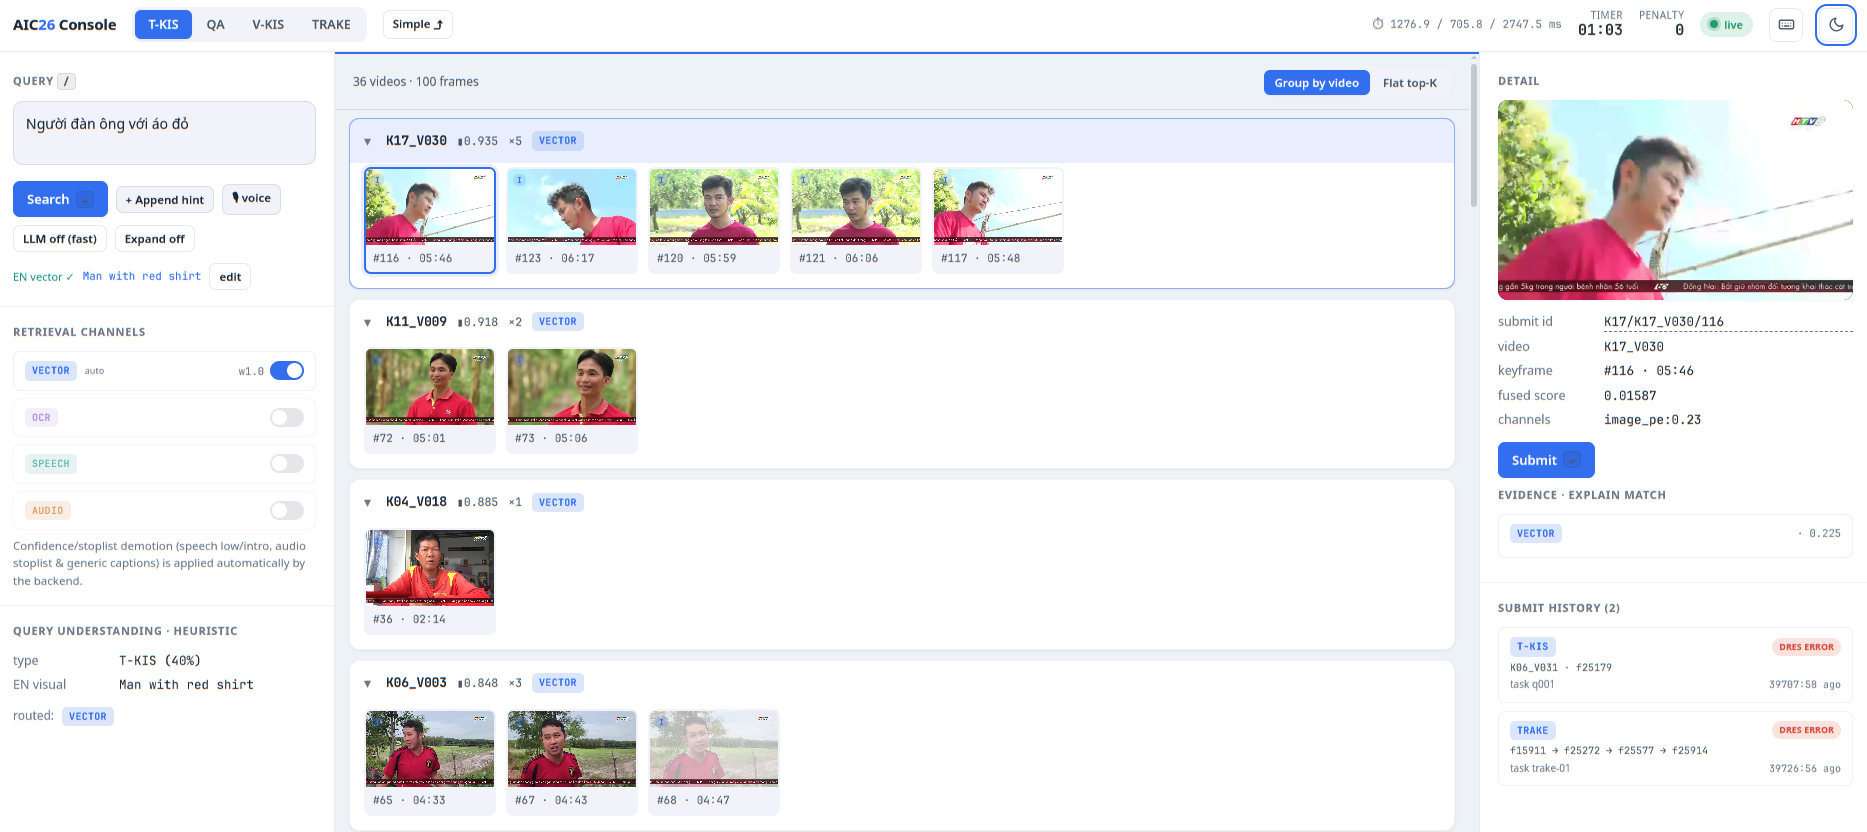
\includegraphics[width=0.98\textwidth]{aic_ui_light.png}
\caption{Operator console for hybrid video retrieval. The interface combines
query routing, grouped keyframe results, inline video playback, timeline
inspection, evidence snippets, and submission controls in a single screen.}
\label{fig:ui-system}
\end{figure*}

\subsection{Evidence Inspection}

Each candidate frame displays channel badges and snippets. OCR evidence includes
clean text and optional clock/hour fields. Speech evidence includes transcript,
time range, confidence bucket, and segment role. Audio evidence includes top
label, caption quality, time range, or GLAP-vector match status. The detail
panel exposes the canonical id, score, timing, keyframe thumbnail, and copyable
identifier.

\subsection{Voice Input and Keyboard Workflow}

The query panel supports browser Web Speech API when available and a backend
Whisper endpoint otherwise. Transcribed Vietnamese text is translated for visual
search when needed. Keyboard shortcuts minimize mouse travel: \texttt{/} focuses
query, \texttt{Enter} searches or opens the guard, arrow keys move between
videos and frames, \texttt{v} opens or hides the video for the selected frame,
\texttt{T} toggles timeline, \texttt{Ctrl+M} starts voice input, and
\texttt{Ctrl+/} opens the shortcut modal.

\subsection{Submission and Duplicate Guard}

The submit guard is the final safety layer. For KIS/V-KIS/QA, the deduplication
key is \texttt{video\_id:frame\_idx}. For TRAKE, it is
\texttt{video\_id|f1,f2,\ldots}. The guard blocks missing frame indices, warns about
duplicates, validates increasing event order, displays evidence, and optionally
creates a local result payload. The current system records this payload in local
history for review and testing; it does not assume an external evaluation
protocol.

\section{Implementation Details}

\subsection{Backend}

The backend is implemented in Python with FastAPI \cite{fastapi2026}. Configuration is loaded from
environment variables or local secret files for development. Core modules are
kept separate from Pydantic/FastAPI request models so ranking logic can be unit
tested independently. Adapter modules wrap Elastic, Milvus, PE text encoding,
and GLAP text encoding. Services implement search, TRAKE, timeline, and
submission history. Mock mode returns deterministic fixtures and is used for
frontend development and automated tests without live services.

Important backend endpoints include \texttt{/api/health}, \texttt{/api/query/parse},
\texttt{/api/search}, \texttt{/api/search/simple}, \texttt{/api/search/trake},
\texttt{/api/videos/\{video\_id\}/timeline}, \texttt{/api/videos/\{video\_id\}/snap},
\texttt{/api/submit}, \texttt{/api/submit/history}, \texttt{/api/translate}, and
\texttt{/api/transcribe}.

\subsection{Frontend}

The frontend is implemented with React, TypeScript, and Vite. It stores no
secrets and talks only to the backend. The main console component owns task
type, query, parser output, selected video/frame, timeline cache, video state,
TRAKE slots, duplicate guard, and submission history. The video viewer seeks to
the selected keyframe timestamp on metadata load and when the selected frame
changes. During TRAKE frame picking, pausing the video captures the raw media
time and thumbnail; the frame index is computed as $\mathrm{round}(t\cdot fps)$,
without snapping back to the nearest extracted keyframe.

\subsection{Storage and Runtime}

Elastic Cloud stores sparse metadata and supports BM25/fuzzy queries. Milvus
stores dense vectors with cosine search. Cloudflare R2 provides public media
URLs. External encoder servers run PE and GLAP text encoders, typically on
Kaggle or a tunnelled inference host. The system exposes health warnings when a
service is unreachable and marks unavailable capabilities in the UI.

\subsection{Operational Readiness Checks}

Before a live session, the deployment verifies that Elastic, Milvus, media, and
encoder endpoints are reachable; indexed document/vector counts match the
expected corpus state; and a sample result carries valid \sid{}, \vid{},
\kfn{}, \ptstime{}, \fid{}, and media URLs. End-to-end checks also confirm that
\texttt{v} opens the selected video at the correct timestamp, the submission
guard blocks duplicates while allowing deliberate overrides, and a TRAKE query
returns an ordered sequence or an explicit partial-result warning.

\section{Experiments and Evaluation}

\subsection{Indexing Statistics}

Table~\ref{tab:index-stats} reports the indexed corpus state. These counts were
derived from the repository staging summary and handoff verification logs.

\begin{table}[t]
\centering
\caption{Indexed corpus statistics.}
\label{tab:index-stats}
\begin{tabular}{lrr}
\toprule
Artifact & Count & Backend \\
\midrule
Videos with temporal maps & 1,478 & Elastic \\
Keyframe map records & 382,299 & Elastic \\
OCR keyframe records & 382,299 & Elastic \\
Speech segments & 48,819 & Elastic \\
Audio windows & 466,996 & Elastic \\
Audio caption records & 35,222 & Elastic \\
PE visual vectors & 382,299 & Milvus \\
GLAP audio vectors & 466,996 & Milvus \\
\bottomrule
\end{tabular}
\end{table}

\subsection{Retrieval Performance on TKIS Queries}

We evaluate the proposed hybrid search approach on the complete TKIS portion of
\texttt{DanhSachTruyVanAIC\_Chungket.xlsx}. It contains 14 final-round queries:
\texttt{tkis-query-01}--\texttt{10} and \texttt{tkis-query-12}--\texttt{15};
identifier 11 is absent from the supplied sheet. Thus, the set was selected only
by task type, rather than by retrieval difficulty or observed performance. To
reflect the sequentially revealed challenge setting, we run one mode with the
full query and another with its first two sentences. The baseline is standalone
CLIP-ViT-H-14 retrieval over the same extracted keyframe corpus.

\subsubsection{Evaluation Protocol}

Each query has one manually annotated target \vid{}. Ground truth is therefore
video-level, not an exact keyframe or temporal interval. Both methods first
retrieve frame candidates, but Recall@K (R@K) is computed on the ranked video
groups after grouping. A query is successful at $K$ when its target \vid{}
occurs among the first $K$ groups. Any extracted keyframe from that video counts
as a hit; retrieving a nearby or different frame in the correct video is not
penalized. Consequently, these numbers measure target-video retrieval and must
not be interpreted as exact-frame localization accuracy. For both methods, up
to 100 frame candidates are retrieved per active channel before grouping, and
the list is not truncated by the UI's display limit before metric computation.
The standalone baseline is grouped with the same video aggregation function so
that $K$ has the same unit for both methods.

The workbook's supplied English translation is used as the visual-text query,
while the original Vietnamese text is used for deterministic channel routing and
for OCR and speech search; no online machine translation is used in the reported
TKIS evaluation. Query type is fixed to TKIS. The heuristic parser is used for
all queries; LLM parsing and visual query expansion are disabled. PE visual
retrieval is always active with weight 1.0. OCR, speech, and audio are activated
only when their deterministic cue rules fire, with weights 0.8, 0.8, and 0.7,
respectively; they are not forced on for every query. Each active channel returns
at most 100 frame hits. Frame lists are fused by weighted RRF with $k=60$, then
grouped using best-frame, top-three-mean, and local temporal-support weights of
0.75, 0.15, and 0.10. Relevance feedback, manual channel overrides, and all
operator interaction are disabled. The first-two-sentences condition applies
the same truncation to the Vietnamese query and its supplied English
translation. This fixed configuration is used for every row in
Table~\ref{tab:tkis-results}; with 14 queries, one query corresponds to 7.14
percentage points.

\begin{table*}[t]
\centering
\caption{Video-level retrieval performance after grouping on all 14 TKIS queries.}
\label{tab:tkis-results}
\scriptsize
\resizebox{0.98\textwidth}{!}{%
\begin{tabular}{lcccccccccc}
\toprule
\multirow{2}{*}{Method} &
\multicolumn{5}{c}{Full Query} &
\multicolumn{5}{c}{First Two Sentences Query} \\
\cmidrule(lr){2-6}\cmidrule(lr){7-11}
& R@1 & R@5 & R@10 & R@50 & R@100
& R@1 & R@5 & R@10 & R@50 & R@100 \\
\midrule
\textbf{Hybrid Search (ours)}
& \textbf{78.57\%} & \textbf{85.71\%} & \textbf{85.71\%}
& \textbf{92.86\%} & \textbf{100.00\%}
& \textbf{64.29\%} & \textbf{85.71\%} & \textbf{92.86\%}
& \textbf{100.00\%} & \textbf{100.00\%} \\
CLIP-ViT-H-14 (standalone)
& 50.00\% & 71.43\% & 78.57\% & 85.71\% & 85.71\%
& 21.43\% & 57.14\% & 57.14\% & 78.57\% & 85.71\% \\
\bottomrule
\end{tabular}
}
\end{table*}

\begin{figure}[!t]
\centering
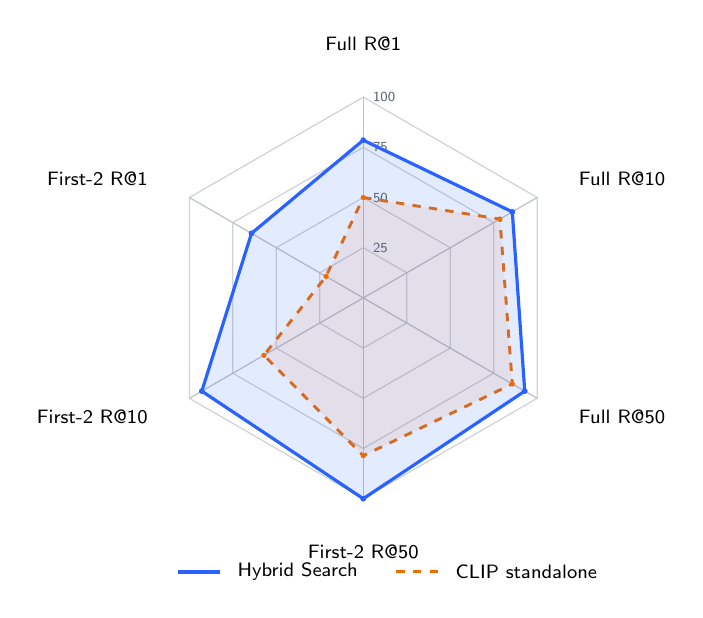
\begin{tikzpicture}
  \def\RadarRadius{2.55}

  \foreach \scale/\tick in {0.25/25,0.50/50,0.75/75,1.00/100} {
    \draw[aicgray!28, line width=0.45pt]
      (90:{\RadarRadius*\scale}) -- (30:{\RadarRadius*\scale}) --
      (-30:{\RadarRadius*\scale}) -- (-90:{\RadarRadius*\scale}) --
      (-150:{\RadarRadius*\scale}) -- (150:{\RadarRadius*\scale}) -- cycle;
    \node[font=\sffamily\tiny, text=aicgray, anchor=west]
      at (90:{\RadarRadius*\scale}) {\tick};
  }

  \foreach \angle in {90,30,-30,-90,-150,150} {
    \draw[aicgray!38, line width=0.45pt] (0,0) -- (\angle:\RadarRadius);
  }

  \node[font=\sffamily\scriptsize, anchor=south] at (90:3.02) {Full R@1};
  \node[font=\sffamily\scriptsize, anchor=west] at (30:3.02) {Full R@10};
  \node[font=\sffamily\scriptsize, anchor=west] at (-30:3.02) {Full R@50};
  \node[font=\sffamily\scriptsize, anchor=north] at (-90:3.02) {First-2 R@50};
  \node[font=\sffamily\scriptsize, anchor=east] at (-150:3.02) {First-2 R@10};
  \node[font=\sffamily\scriptsize, anchor=east] at (150:3.02) {First-2 R@1};

  \path[draw=aicorange, draw opacity=1, fill=aicorange, fill opacity=0.09,
    dashed, line width=1.05pt]
    (90:{\RadarRadius*0.5000}) --
    (30:{\RadarRadius*0.7857}) --
    (-30:{\RadarRadius*0.8571}) --
    (-90:{\RadarRadius*0.7857}) --
    (-150:{\RadarRadius*0.5714}) --
    (150:{\RadarRadius*0.2143}) -- cycle;

  \path[draw=aicblue, draw opacity=1, fill=aicblue, fill opacity=0.13,
    line width=1.15pt]
    (90:{\RadarRadius*0.7857}) --
    (30:{\RadarRadius*0.8571}) --
    (-30:{\RadarRadius*0.9286}) --
    (-90:{\RadarRadius*1.0000}) --
    (-150:{\RadarRadius*0.9286}) --
    (150:{\RadarRadius*0.6429}) -- cycle;

  \foreach \angle/\value in {90/0.7857,30/0.8571,-30/0.9286,
      -90/1.0000,-150/0.9286,150/0.6429} {
    \fill[aicblue] (\angle:{\RadarRadius*\value}) circle (1.05pt);
  }
  \foreach \angle/\value in {90/0.5000,30/0.7857,-30/0.8571,
      -90/0.7857,-150/0.5714,150/0.2143} {
    \fill[aicorange] (\angle:{\RadarRadius*\value}) circle (0.95pt);
  }

  \draw[aicblue, line width=1.15pt] (-2.35,-3.48) -- (-1.82,-3.48);
  \node[font=\sffamily\scriptsize, anchor=west] at (-1.72,-3.48)
    {Hybrid Search};
  \draw[aicorange, dashed, line width=1.05pt] (0.42,-3.48) -- (0.95,-3.48);
  \node[font=\sffamily\scriptsize, anchor=west] at (1.05,-3.48)
    {CLIP standalone};
\end{tikzpicture}
\caption{Retrieval profiles on the 14 TKIS queries at selected cutoffs. Each
spoke reports video-level Recall@K (\%); First-2 denotes the first-two-sentences
condition.}
\label{fig:tkis-radar}
\end{figure}

Table~\ref{tab:tkis-results} reports the exact values, while
Fig.~\ref{fig:tkis-radar} summarizes selected cutoffs as retrieval profiles.
The results show a consistent advantage for the hybrid system over the
standalone CLIP baseline. Under full-query evaluation, hybrid
search improves early retrieval most strongly: R@1 increases from 50.00\% to
78.57\%, meaning that the correct target video becomes the first group for four
more queries out of 14. The gain remains visible at larger cutoffs, reaching
92.86\% at R@50 and full recall at R@100. This pattern suggests that combining
visual-text embeddings with selectively routed OCR, speech, and audio evidence,
followed by rank fusion and video grouping, reduces early-ranking mistakes while
keeping broad recall.

The incomplete-query setting makes the robustness difference clearer. When only
the first two sentences are used, standalone CLIP drops sharply to 21.43\% R@1,
while hybrid search sustains 64.29\% R@1 and reaches 100.00\% by R@50. This is
important for interactive search because operators often issue an initial query
before all query details are fully processed. Auxiliary modalities help recover
from missing context: OCR can match visible names and numbers, metadata can
anchor likely videos or time ranges, and speech or audio evidence can contribute
when the query contains those cues. The result should still be interpreted
cautiously because the evaluation set is small and modality-level ablations are
not yet reported. In particular, this table does not isolate or attribute gains
to the optional caption and object enrichment extensions. The observed trend
supports multimodal fusion over a standalone visual-text baseline.

\subsection{TRAKE Retrieval Evaluation}
\label{sec:trake-eval}

The supplied workbook contains four TRAKE queries, and we evaluate the complete
set rather than a selected subset. Because it does not include machine-readable
target frames, each first-ranked result is manually inspected. A query is counted
as correct at R@1 only when the top-ranked video contains one visually matching
frame for every described event and the selected timestamps are strictly
increasing. Table~\ref{tab:trake-results} reports 4/4 correct first-ranked
sequences and full coverage of all 14 events. This is an operator-verified
sequence-level result on a small set, not an official test-server score.

\begin{table}[!t]
\centering
\caption{Operator-verified TRAKE performance on all supplied queries. Event
coverage is measured within the first-ranked sequence.}
\label{tab:trake-results}
\scriptsize
\setlength{\tabcolsep}{2pt}
\begin{tabularx}{\columnwidth}{@{}>{\ttfamily\raggedright\arraybackslash}p{0.18\columnwidth}Xcc@{}}
\toprule
Query & Ordered event scenario & Events & R@1 / coverage \\
\midrule
trake-01 & Character-costume appearances & 4 & Correct; 4/4 \\
trake-02 & Cycling finish order & 3 & Correct; 3/3 \\
trake-03 & Philippines--Brunei match events & 3 & Correct; 3/3 \\
trake-04 & Cooking ingredient order & 4 & Correct; 4/4 \\
\midrule
Overall & All supplied TRAKE queries & 14 & 4/4; 14/14 \\
\bottomrule
\end{tabularx}
\end{table}

\textit{Controlled greedy-failure trace.} Table~\ref{tab:trake-controlled}
evaluates the specific failure mode targeted by the sequence DP using a
controlled three-event candidate trace. The greedy baseline takes the
highest-scoring candidate for each event that remains later than its previous
pick. It chooses $E_1$ at 50~s and $E_2$ at 70~s, leaving no valid candidate for
$E_3$ at 60~s. The proposed DP selects the lower-scoring early candidates at
10~s and 30~s, then reaches $E_3$ at 60~s. This fixture is executed by the same
backend sequence assembler in the unit tests.

\begin{table}[!t]
\centering
\caption{Controlled synthetic TRAKE trace. Scores in parentheses are retrieved
candidate relevance. The example validates greedy failure, not corpus-level
TRAKE accuracy.}
\label{tab:trake-controlled}
\scriptsize
\setlength{\tabcolsep}{2pt}
\begin{tabularx}{\columnwidth}{@{}>{\raggedright\arraybackslash}p{0.21\columnwidth}XXXX@{}}
\toprule
Method & $E_1$ & $E_2$ & $E_3$ & Valid order / coverage \\
\midrule
Greedy & 50~s (0.95) & 70~s (0.93) & -- & No; $2/3$ \\
Proposed DP & 10~s (0.80) & 30~s (0.83) & 60~s (0.90) & Yes; $3/3$ \\
\bottomrule
\end{tabularx}
\end{table}

The controlled result demonstrates that temporal coverage can require rejecting
a locally stronger earlier event. Broader TRAKE conclusions still require a
held-out set with machine-readable video and event-time annotations, comparison
against retrieval baselines, and repeated live runs for end-to-end latency.

\subsection{Backend Runtime Diagnostics}

Table~\ref{tab:runtime} reports warm backend latency on the live deployment.
Each retrieval operation uses one warm-up followed by 25 measured requests with
100 candidates per active channel. Table~\ref{tab:runtime} reports median,
nearest-rank p95, and min--max wall-clock latency from the backend host. The
local heuristic router remains below 0.1~ms over 100 calls and is omitted from
the table. The full-hybrid row activates PE, OCR, speech, and Elastic+GLAP audio
concurrently and includes timing enrichment, weighted RRF, and video grouping.
The accompanying \texttt{benchmark\_runtime.py} runner uses fixed channel queries
and excludes parser and translation overhead. External service load and network
conditions are therefore part of all measurements.

\begin{table}[!t]
\centering
\caption{Warm backend latency on the live deployment ($n=25$ measured requests
per retrieval operation after one warm-up).}
\label{tab:runtime}
\scriptsize
\setlength{\tabcolsep}{2.5pt}
\begin{tabularx}{\columnwidth}{@{}Xrrr@{}}
\toprule
Operation & Median & p95 & Min--max \\
\midrule
PE visual retrieval & 1.38 s & 1.64 s & 1.33--1.66 s \\
OCR retrieval & 1.65 s & 2.17 s & 1.60--2.69 s \\
Speech retrieval & 1.64 s & 2.64 s & 1.60--3.02 s \\
Audio retrieval & 2.51 s & 2.97 s & 2.42--3.12 s \\
Full four-channel hybrid & \textbf{2.55 s} & \textbf{3.36 s} & 2.48--4.38 s \\
\bottomrule
\end{tabularx}
\end{table}

These values characterize service responsiveness, not human search efficiency.
Browser video open/seek latency, time-to-correct-result, duplicate attempts, and
wrong-frame selections were not instrumented in this evaluation.

\subsection{Module Validation}

The project validates modules at several levels. Upload scripts include unit
tests for keyframe mapping, Elastic document construction, OCR normalization,
Milvus entity schemas, and retry behavior. Backend tests cover identity parsing,
media URL construction, query parsing, scoring demotions, RRF fusion,
group-by-video ranking, TRAKE dynamic programming, adapter mock behavior,
timeline construction, duplicate submission blocking, translation fallback, and
API responses. Frontend component tests cover search flow, grouped and flat
views, keyboard selection, video toggle with \texttt{v}, TRAKE quick submit,
duplicate guard, and simple vector search.

Extraction-specific validation was performed without exhaustive manual labels.
For keyframe extraction, validation checks map-file monotonicity, valid
\fid{} and \ptstime{} ranges, stability-score distributions, duplicate rates
after temporally decayed coverage, and successful joins from extracted frames to
media URLs. For OCR, the pipeline verified 382,299 unique records with no
duplicate ids and tracked the reduction from cleanup. For speech, alignment
confidence distributions were inspected and low-score segments were preserved
for indexing time demotion. For audio, window integrity was checked across 1,478
videos, and tag/caption quality analysis motivated stoplists and caption-quality
fields. For structured captions, validation focuses on JSON parse rate,
hard-field vocabulary coercion, near-duplicate inheritance, and spot checks of
text-independent V-KIS fields. For object detection, weak validation compares
overlapping classes with provided object metadata where available, measures
cross-detector agreement, and renders bbox overlays for genre-vocabulary and
threshold tuning.

\subsection{Retrieval Case Studies}

The aggregate evaluation retained Recall@K values but not its original
per-query rank log. After restoring the PE encoder, we therefore reran four
post-hoc cases with the fixed protocol above: 100 candidates per active channel,
weighted RRF, video grouping, and no feedback, expansion, or manual override.
Targets were verified independently from indexed OCR, speech, or audio evidence.
The additional speech diagnostic was constructed from a distinctive fact in an
indexed ASR segment to isolate the speech channel; it is not one of the 14
official TKIS queries. Table~\ref{tab:verified-cases} reports actual PE-only and
full-hybrid video-group ranks from this rerun. These cases explain individual
behavior but are not an additional aggregate benchmark.

\begin{table}[!t]
\centering
\caption{Verified retrieval cases from a post-hoc live rerun. V/H denote
PE-only and full-hybrid video-group ranks; the speech and audio diagnostics are
outside the 14-query quantitative set.}
\label{tab:verified-cases}
\scriptsize
\setlength{\tabcolsep}{2pt}
\begin{tabularx}{\columnwidth}{@{}>{\raggedright\arraybackslash}p{0.18\columnwidth}>{\raggedright\arraybackslash}p{0.28\columnwidth}X@{}}
\toprule
Case & Target and observed rank & Query cue and decisive evidence \\
\midrule
OCR (TKIS-03) & \texttt{K13\_V001}/016; V $>$100 $\rightarrow$ H 68 &
The query asks for stage 01 of the television cycling race in Tuyên Quang. OCR
reads ``ĐOÀN ĐUA CÚP TRUYỀN HÌNH ĐẾN TUYÊN QUANG,'' bringing an otherwise missed
target into the top 100. \\
Speech (TKIS-09) & \texttt{K14\_V025}/202; V 11 $\rightarrow$ H 11 &
The query describes villagers in Indonesia sleeping on sand. ASR at
595.2--615.4 s mentions a rural village on Madura island, Indonesia, and the
long-standing practice of sleeping on sand. \\
Speech diagnostic & \texttt{K06\_V005}/196; V 28 $\rightarrow$ H 12 &
``Lời thuyết minh nói lễ hội bắt nguồn từ một lễ hội tôn giáo vào thế kỷ thứ
mười chín để tôn vinh Đức Mẹ Maria.'' ASR at 763.878--788.153 s states this
origin explicitly, improving the target by 16 video-group positions. \\
Audio diagnostic & \texttt{L24\_V023}/047; V 19 $\rightarrow$ H 15 &
``Tiếng chuông kim loại vang liên tục, đều nhịp.'' The 162.5--167.5 s window has
label \texttt{Bell} and a caption describing continuous rhythmic metallic
ringing resembling a bell or gong. \\
\bottomrule
\end{tabularx}
\end{table}

The OCR case is a genuine rescue at the R@100 cutoff: PE alone does not return
the target, whereas the location-specific title makes it reachable through OCR.
The official TKIS speech case does not improve the video rank and is reported as
such; instead, it changes the representative evidence from a visually plausible
frame to a transcript-backed moment, making verification less ambiguous. The
separate speech diagnostic improves the target from rank 28 to 12 because its
defining fact is spoken rather than visually observable. Since this query was
formed from inspected ASR evidence, the result demonstrates channel behavior but
must not be treated as an unbiased benchmark gain. The audio case improves the
target by four positions, but is likewise labeled as a diagnostic probe because
none of the 14 supplied TKIS descriptions defines a sound event as its target.
These cases expose both gains and non-gains rather than attributing every
successful query to multimodal fusion.

\subsection{Planned Ablation Protocol}

Table~\ref{tab:ablation} defines a planned ablation protocol for future held-out
evaluation. No quantitative ablation results are claimed in this work. Because
official competition ground truth is not part of this repository, these ablations
are suitable for a future validation set of KIS/QA/TRAKE tasks.

\begin{table}[!t]
\centering
\caption{Recommended future ablations.}
\label{tab:ablation}
\scriptsize
\setlength{\tabcolsep}{2pt}
\begin{tabularx}{\columnwidth}{@{}>{\raggedright\arraybackslash}p{0.20\columnwidth}>{\raggedright\arraybackslash}p{0.31\columnwidth}X@{}}
\toprule
Variant & Removed component & Hypothesis (not measured) \\
\midrule
Visual only & Dense PE without OCR/speech/audio & Misses exact text, spoken phrases, and sound cues \\
No OCR & Remove OCR channel from full system & Lower recall for lower-thirds, signage, names, numbers, clocks \\
No speech & Remove ASR channel & Lower recall for spoken descriptions and QA evidence \\
No audio vector & Keep Elastic audio tags/captions, remove GLAP & Lower recall for semantic sound queries and noisy tags \\
No grouping & Show flat fused frames only & Repeated videos may increase inspection effort \\
Old count-heavy grouping & Replace best-frame-dominant score & Videos with many mediocre frames overtake strong candidates \\
Greedy TRAKE & Replace DP with left-to-right greedy picks & Locally strong early event can block a globally valid sequence \\
No submit guard & Submit directly from selected result & Duplicate and wrong-frame risk may increase \\
\bottomrule
\end{tabularx}
\end{table}

\section{Limitations and Future Work}

\textbf{No controlled interaction study.} Keyboard navigation, grouped video
results, timeline inspection, and the submission guard are implemented and
covered by functional tests, but this paper does not measure their human-facing
effect. In particular, no flat-versus-grouped comparison, guard ablation, or
multi-operator study reports time-to-correct-result, duplicate attempts, or
wrong-frame selections. We therefore treat these components as system features,
not as experimentally established improvements to live search performance.

\textbf{No official test-server score or retained TKIS per-query log.}
Table~\ref{tab:tkis-results}
is an internal video-level evaluation over the supplied final-round TKIS list;
it is not an official leaderboard result, and its original run retained
aggregate Recall@K rather than per-query ranks. A future paper version should
persist the full ranked lists and report MRR,
Recall@K, successful submission rate, median time-to-correct-submit, and
wrong-submit rate on a task suite.

\textbf{No live VLM reranker or visual QA chain-of-thought.} The current system
does not run a top-$k$ VLM reranker or image-based QA reasoning. The backend has
clean extension points for such a reranker, but health flags currently mark
these capabilities as unavailable.

\textbf{Vietnamese analysis remains simple.} Elastic text fields currently use
standard text mappings and folded fields rather than a custom Vietnamese
analyzer. This is robust enough for many queries but may underperform on
morphologically complex or diacritic-error cases.

\textbf{Audio labels are noisy.} CED tags include systematic errors on
Vietnamese speech. Stoplists and demotions reduce but do not eliminate this
noise. GLAP provides a second retrieval path, but GLAP availability depends on
the external encoder endpoint.

\textbf{Video loading performance.} Inline video loading depends on remote MP4
layout and network behavior. Remuxing videos with fast-start metadata, adding
lower-bitrate preview proxies, and delaying timeline thumbnails until video
metadata is ready would improve operator latency.

\textbf{Caption/object accuracy lacks labeled evaluation.} The keyframe
extractor is part of the offline corpus construction used by the retrieval
system, while captioning and object grounding are enrichment branches over the
same extracted frame registry. Their remaining limitation is evaluation and
serving depth: without exhaustive caption/object labels, the paper reports
schema design, weak validation, and integration contracts rather than mAP or
caption-relevance scores.

\section{Conclusion}

This paper presented \sys{} as an adaptive-keyframe and evidence-aware hybrid
retrieval system for AIC 2026. The offline method constructs representative
frames while preserving a canonical frame-time identity across visual, OCR,
speech, and audio indices. Online cue routing, weighted RRF, and video grouping
raise full-query video-level R@1 from 50.00\% to 78.57\% over the standalone
baseline and retain a larger advantage when query text is truncated. The TRAKE
branch further uses exact dynamic programming for globally ordered event
assembly; all four supplied TRAKE queries return an operator-verified correct
sequence at R@1, with 14/14 event coverage. Across 25 post-warm-up requests, the
four-channel hybrid path records 2.55 s median and 3.36 s p95 backend latency.
The interface, timeline, grouping workflow, and submission guard complete the
deployed system, but their effects on search time and submission errors require
a controlled multi-operator study before making interaction-performance claims.

\IEEEtriggeratref{16}
\bibliographystyle{IEEEtran}
\bibliography{references}

\end{document}
